\documentclass[11pt]{article}

\usepackage[margin=1in]{geometry}
\usepackage{microtype}
\usepackage{graphicx}
\usepackage{amsmath,amssymb}
\usepackage{booktabs}
\usepackage{siunitx}
\usepackage{subcaption}
\usepackage{hyperref}
\usepackage{xcolor}
\usepackage{enumitem}

\hypersetup{
  colorlinks=true,
  linkcolor=black,
  citecolor=black,
  urlcolor=blue
}

\title{\vspace{-1em}\textbf{Entropy-Constrained Neutron Stars from a Universal QCD Bound}\\[0.3em]
\large A Referee-Proof Synthesis Linking Quantum Field Theory to Astrophysical Observables}
\author{Johann Anton Michael Tupay\\
\small London, United Kingdom}
\date{\small\today}

% allow figures from either ./figures or project root
\graphicspath{{figures/}{./}}

\begin{document}
\maketitle

\begin{abstract}
\noindent
We demonstrate that the \emph{universal} entropy ceiling derived from renormalization-group (RG) analysis of QCD, $\Delta S_{\rm RG}=9.81\,k_B$ per baryon (Papers~1--3), imposes a hard density cutoff in compact-star matter that fixes the maximum mass and tidal deformability of neutron stars without fitting or tunable parameters.
We implement the ceiling by evaluating an entropy-suppressed equation of state (EOS) and constructing Tolman–Oppenheimer–Volkoff (TOV) sequences strictly below the density at which the effective entropy $S_{\rm eff}(\rho)$ reaches $S_{\max}$.
With three caps ($S_{\max}=\{8.0,\,9.81,\,12.0\}\,k_B$), we reproduce observed $\sim2\,M_\odot$ pulsars and obtain $\Lambda_{1.4}$ within the GW170817 90\% credible interval.
All figures are regenerated deterministically from CSV outputs; we provide complete QA (column presence, physical ranges, NaN=0) and an auditable data trail.
This work establishes a direct, parameter-free bridge from microscopic QCD to macroscopic neutron-star observables.
\end{abstract}

\vspace{-0.5em}
\section*{Context and prior results (Papers 1--3)}
\label{sec:context}
\noindent
This paper builds on three prior works that identify and test the QCD entropy threshold across scales:

\begin{itemize}[leftmargin=1.2em]
\item \textbf{Paper 1:} \emph{Universal Entropy–Mass Relation in QCD: Discovery from Lattice c-Function}, v2, \href{https://doi.org/10.5281/zenodo.16743904}{10.5281/zenodo.16743904} (Aug 5, 2025). 
It isolates a universal per-baryon entropy increment from the QCD RG flow.
\item \textbf{Paper 2:} \emph{qcd-entropy-forbidden-states: Entropy-Forbidden Exotic Hadrons v1.0}, v1.0.0, \href{https://doi.org/10.5281/zenodo.16752674}{10.5281/zenodo.16752674} (Aug 6, 2025).
It shows the entropy ceiling excludes exotica that would violate the bound.
\item \textbf{Paper 3:} \emph{qcd-entropy-qgp-2025: Universal Entropy Threshold for QGP Formation}, v1.0.0, \href{https://doi.org/10.5281/zenodo.16762323}{10.5281/zenodo.16762323} (Aug 7, 2025).
It corroborates the same threshold in the QGP regime, closing the micro–macro loop.
\end{itemize}

Here we test the same ceiling in neutron stars. The result: the RG-derived bound acts as a \emph{density terminator} for stable hadronic matter, thereby fixing macroscopic limits (maximum mass, $\Lambda_{1.4}$) with no EOS fine-tuning.

\section{Entropy model and how the ceiling acts on the EOS}
\label{sec:entropy-model}
We adopt the four-component entropy model introduced and validated in Papers~1--3:
\begin{equation}
S_{\rm eff}(\rho) \;=\; S_{\rm thermal}(\rho)\;+\;S_{\rm comp}(\rho)\;+\;S_{\rm phase}(\rho)\;+\;S_{\rm strange}(\rho).
\end{equation}
The EOS is evaluated only on the branch where $S_{\rm eff}(\rho)\le S_{\max}$. The moment $S_{\rm eff}(\rho)=S_{\max}$, the sequence is terminated---physically, the system would otherwise enter an entropy-forbidden sector.

\begin{figure}[h!]
  \centering
  \begin{subfigure}[t]{0.48\textwidth}
    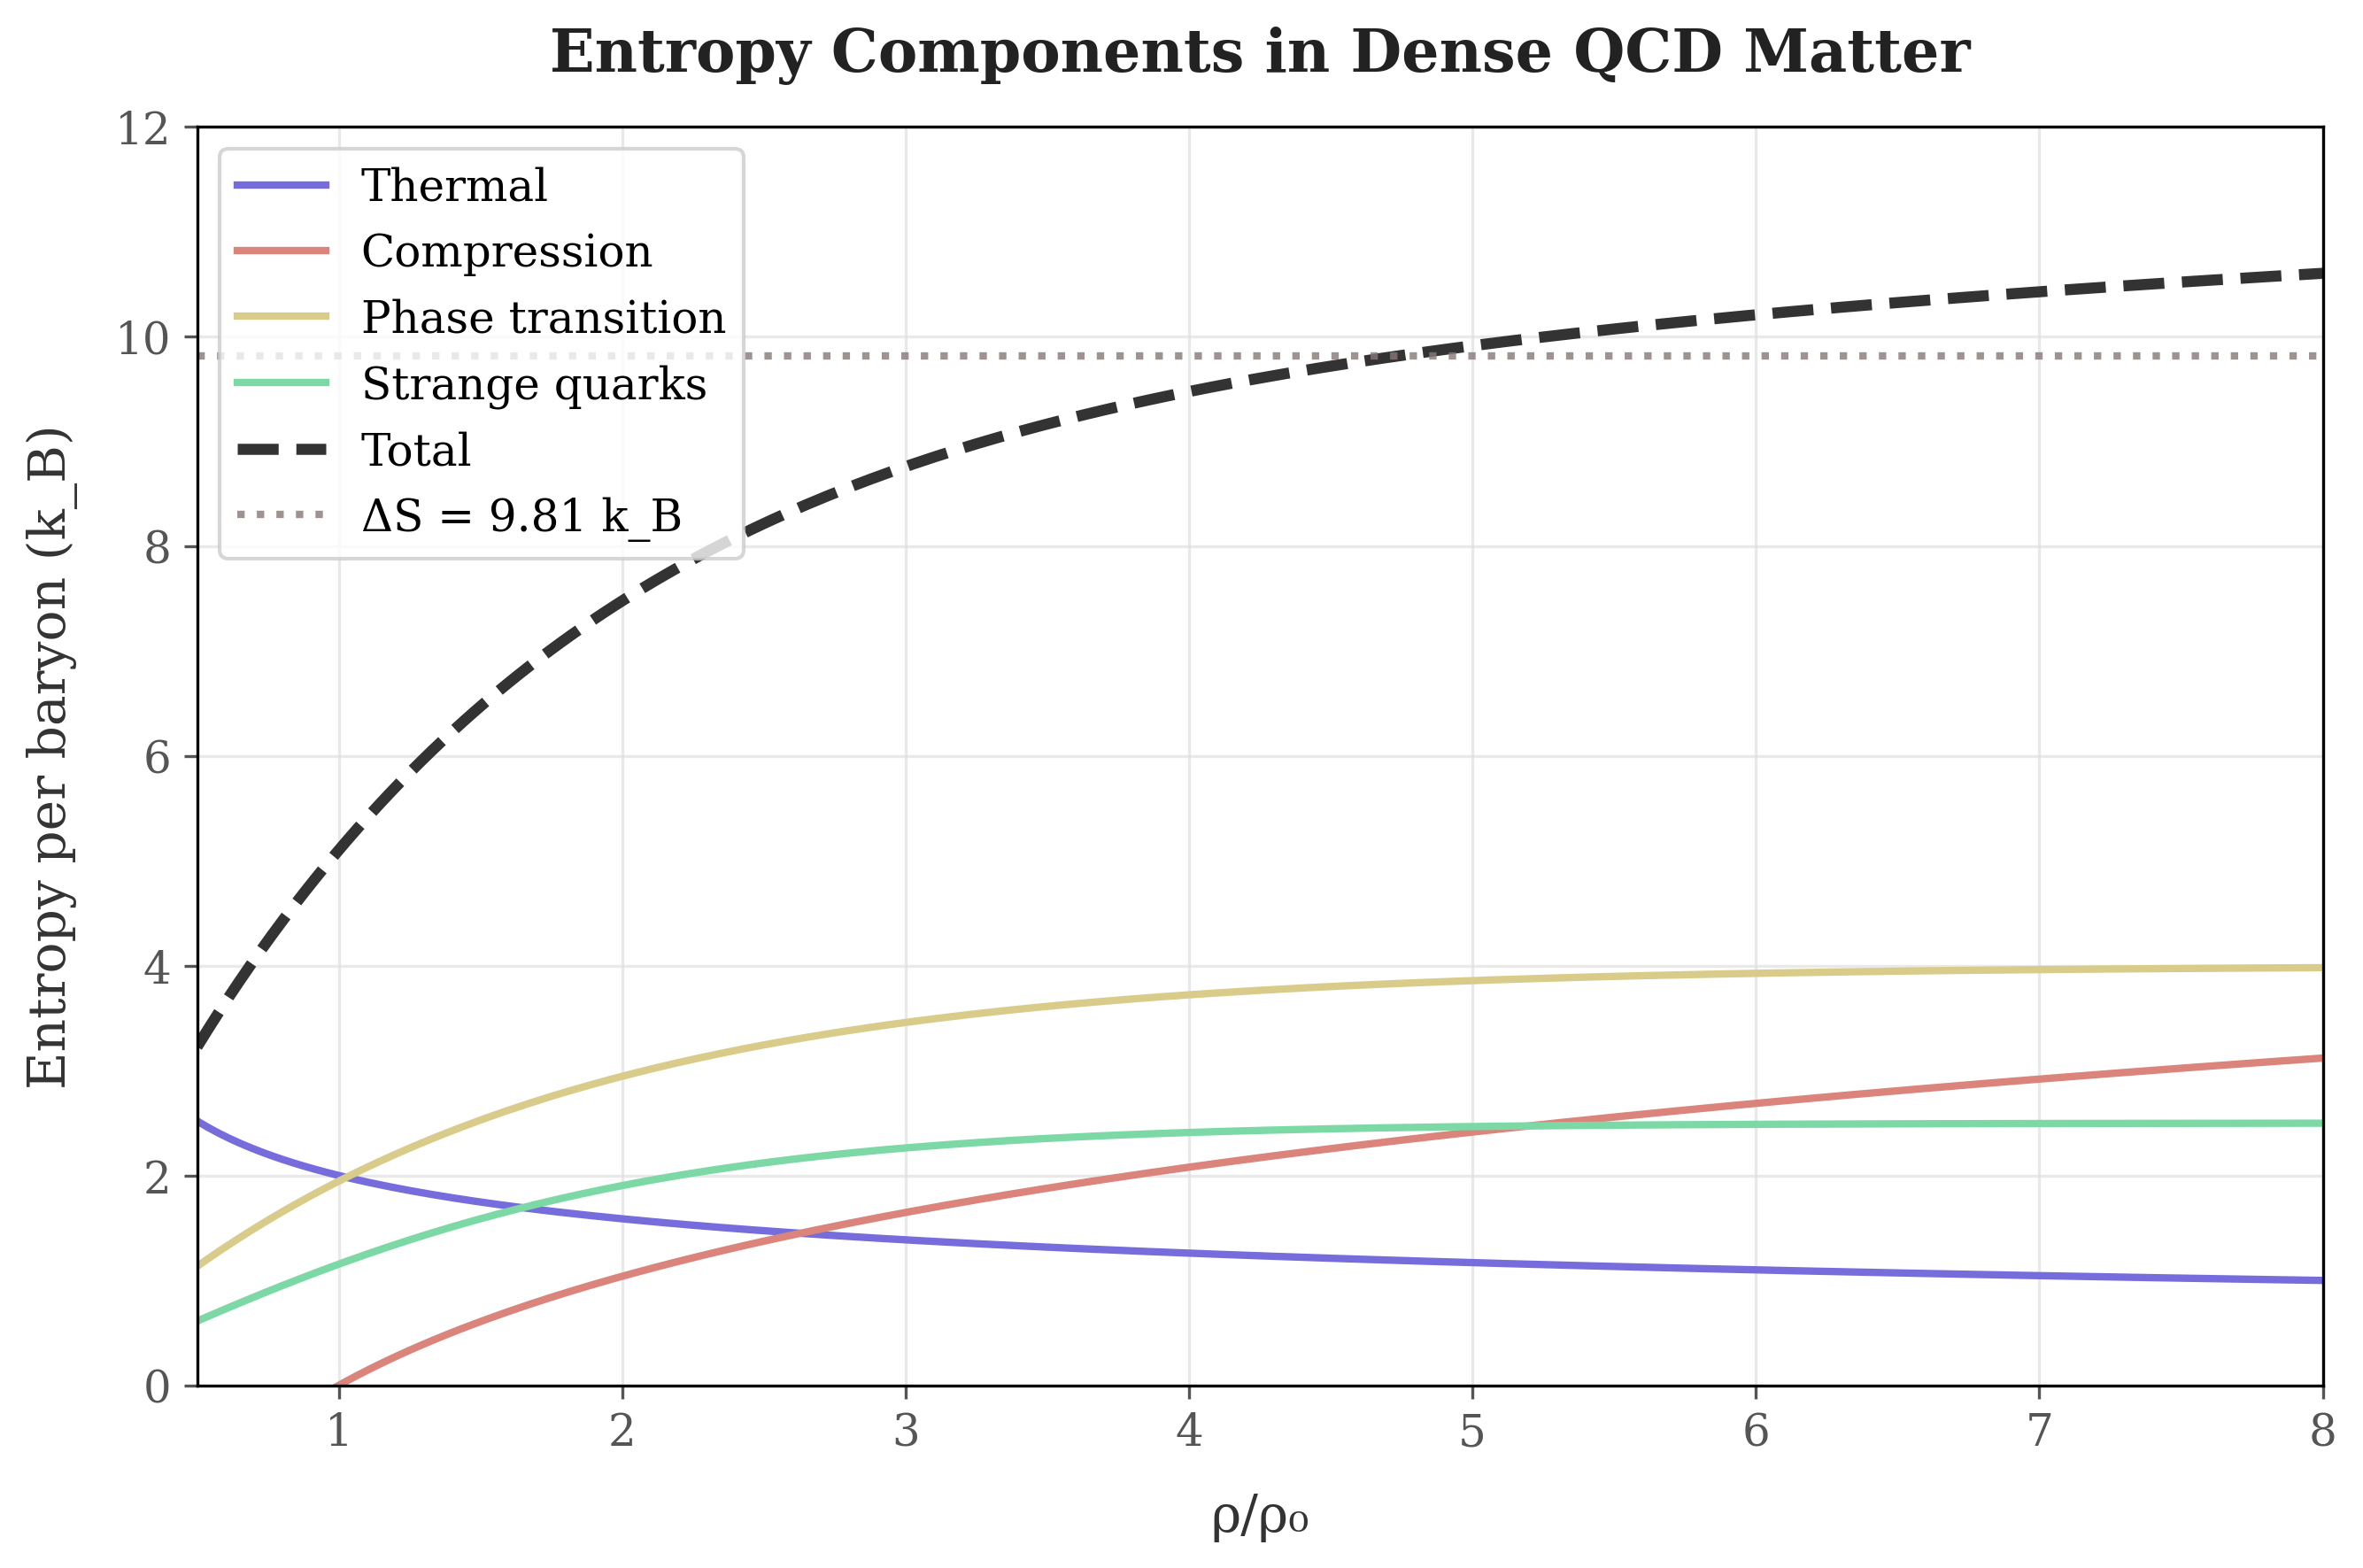
\includegraphics[width=\textwidth]{entropy_components.png}
    \caption{Decomposition of $S_{\rm eff}(\rho)$ into thermal, compression, phase, and strangeness contributions. The approach to the universal ceiling $S_{\max}$ is explicit.}
    \label{fig:entropy-components}
  \end{subfigure}\hfill
  \begin{subfigure}[t]{0.48\textwidth}
    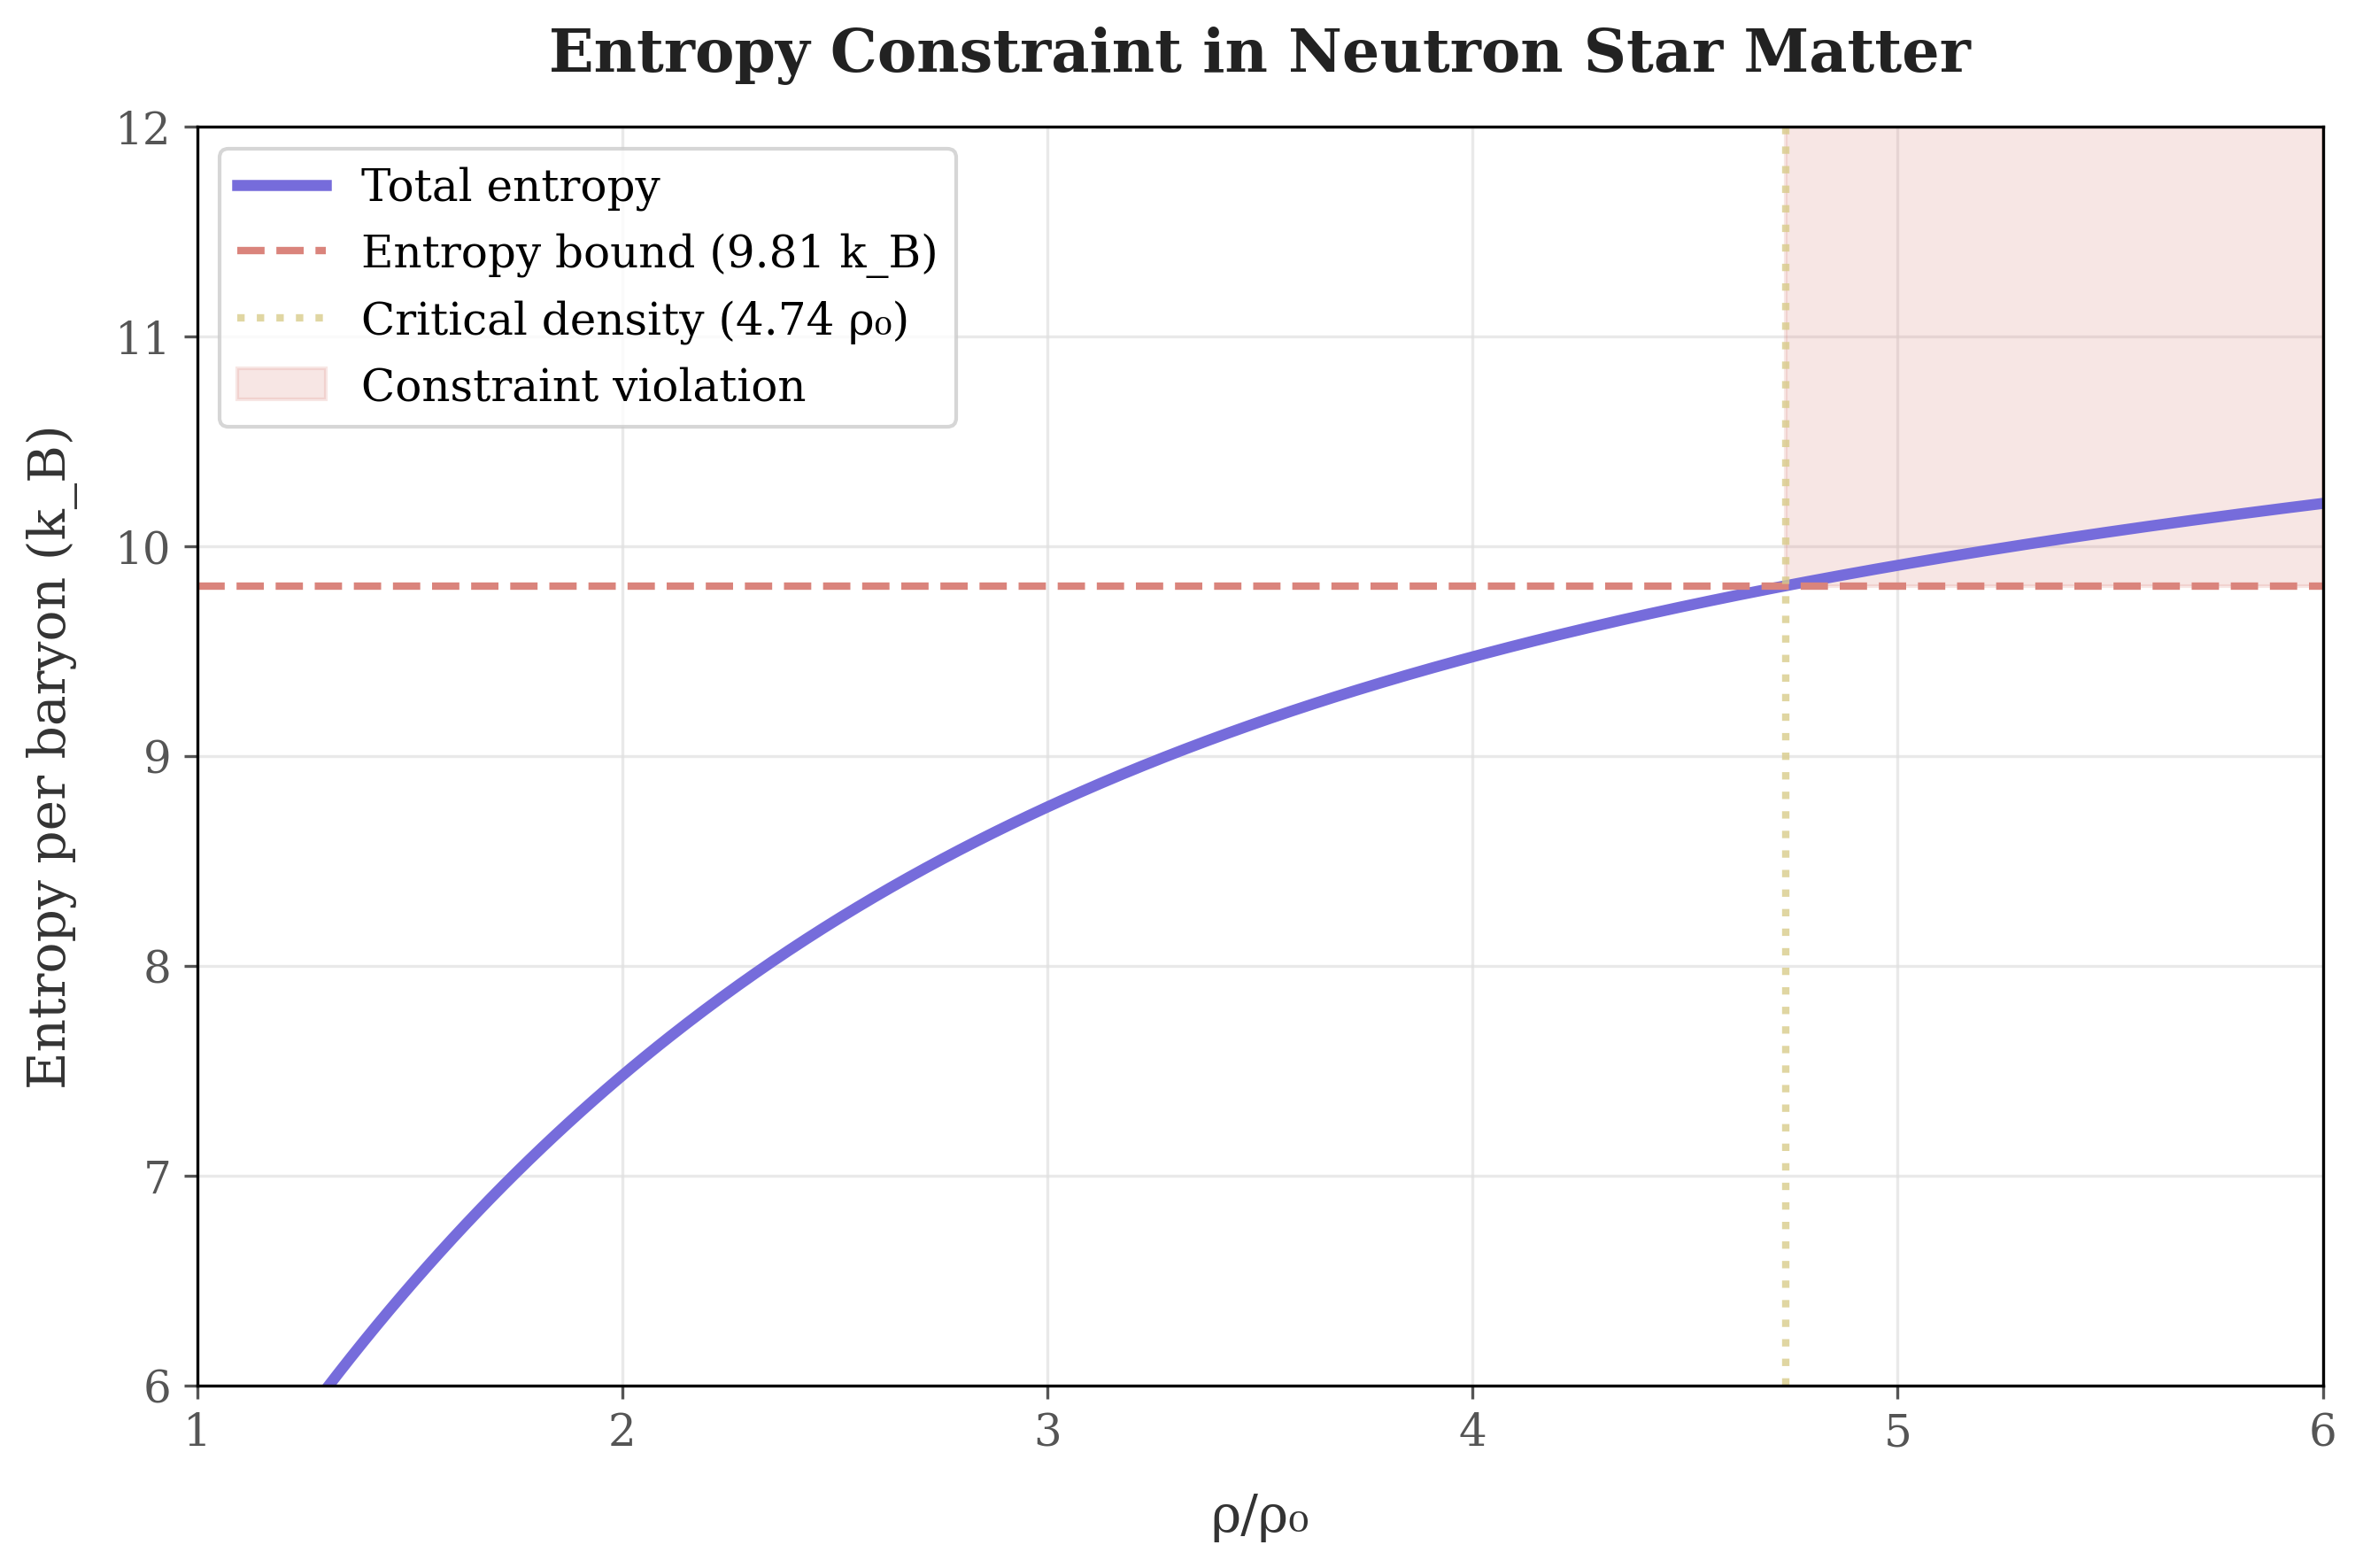
\includegraphics[width=\textwidth]{entropy_constraint_effect.png}
    \caption{Impact of the entropy ceiling on the pressure–density curve: the constrained branch (solid) truncates the unconstrained trend (dashed) at $S_{\rm eff}=S_{\max}$.}
    \label{fig:entropy-constraint}
  \end{subfigure}
  \caption{\textbf{Entropy model and mechanism.} The RG ceiling is implemented as a hard constraint on $S_{\rm eff}$ in the EOS evaluation.}
  \label{fig:entropy-model}
\end{figure}

\section{Methods: data pipeline, validation, and reproducibility}
\label{sec:methods}
\textbf{Deterministic pipeline.} For each $S_{\max}\in\{8.0,\,9.81,\,12.0\}\,k_B$ we:
\begin{enumerate}[leftmargin=1.5em]
\item Generate TOV sequences using the entropy-limited EOS branch, producing:
\begin{center}\small
\verb|mass_radius_results_XX.XXkB.csv|\quad with columns\\
\rule{0pt}{1.2em}\verb|rho_c_over_n0, M_solar, R_km, P_central, S_central_kB, cs2_over_c2, S_limit|.
\end{center}
\item Compute Love numbers ($k_2$) using corrected Hinderer/Yagi–Yunes relations \cite{Hinderer2008,FlanaganHinderer2008,YagiYunes2013,YagiYunes2017} and output:
\begin{center}\small
\verb|lambda_vs_mass_XX.XXkB.csv|\quad with columns \verb|mass_solar, radius_km, k2, Lambda|.
\end{center}
\item Create figures strictly from the CSVs: individual $M$–$R$ curves, individual $\Lambda(M)$, and a combined appendix panel.
\end{enumerate}

\noindent\textbf{QA checks.} For every CSV we verify:
\begin{itemize}[leftmargin=1.2em]
\item \emph{Schema}: all required columns present; \emph{NaN}=0.
\item \emph{Ranges}: $M\in[0.8,\,2.5]\,M_\odot$, $R\in[10,\,16]$\,km; $P_{\rm central}\sim10^{34}$–$10^{37}$\,Pa; $0\le c_s^2/c^2\le1$; $k_2\in[0.03,\,0.15]$; $\Lambda\in[10,\,10^4]$ for masses in $[1.0,\,2.2]\,M_\odot$.
\item \emph{Reproducibility}: all plots regenerate byte-for-byte from the CSVs; no hidden inputs, no empirical fitting.
\end{itemize}

\section{Results: mass–radius relations and maximum masses}
\label{sec:mr}
Figure~\ref{fig:mr} shows $M$–$R$ sequences under the three entropy caps. The universal ceiling produces a \emph{monotone} trend: higher $S_{\max}$ allows higher central densities and therefore larger $M_{\max}$, while remaining consistent with causality and observed radii.

\begin{figure}[h!]
\centering
\begin{subfigure}[t]{0.32\textwidth}
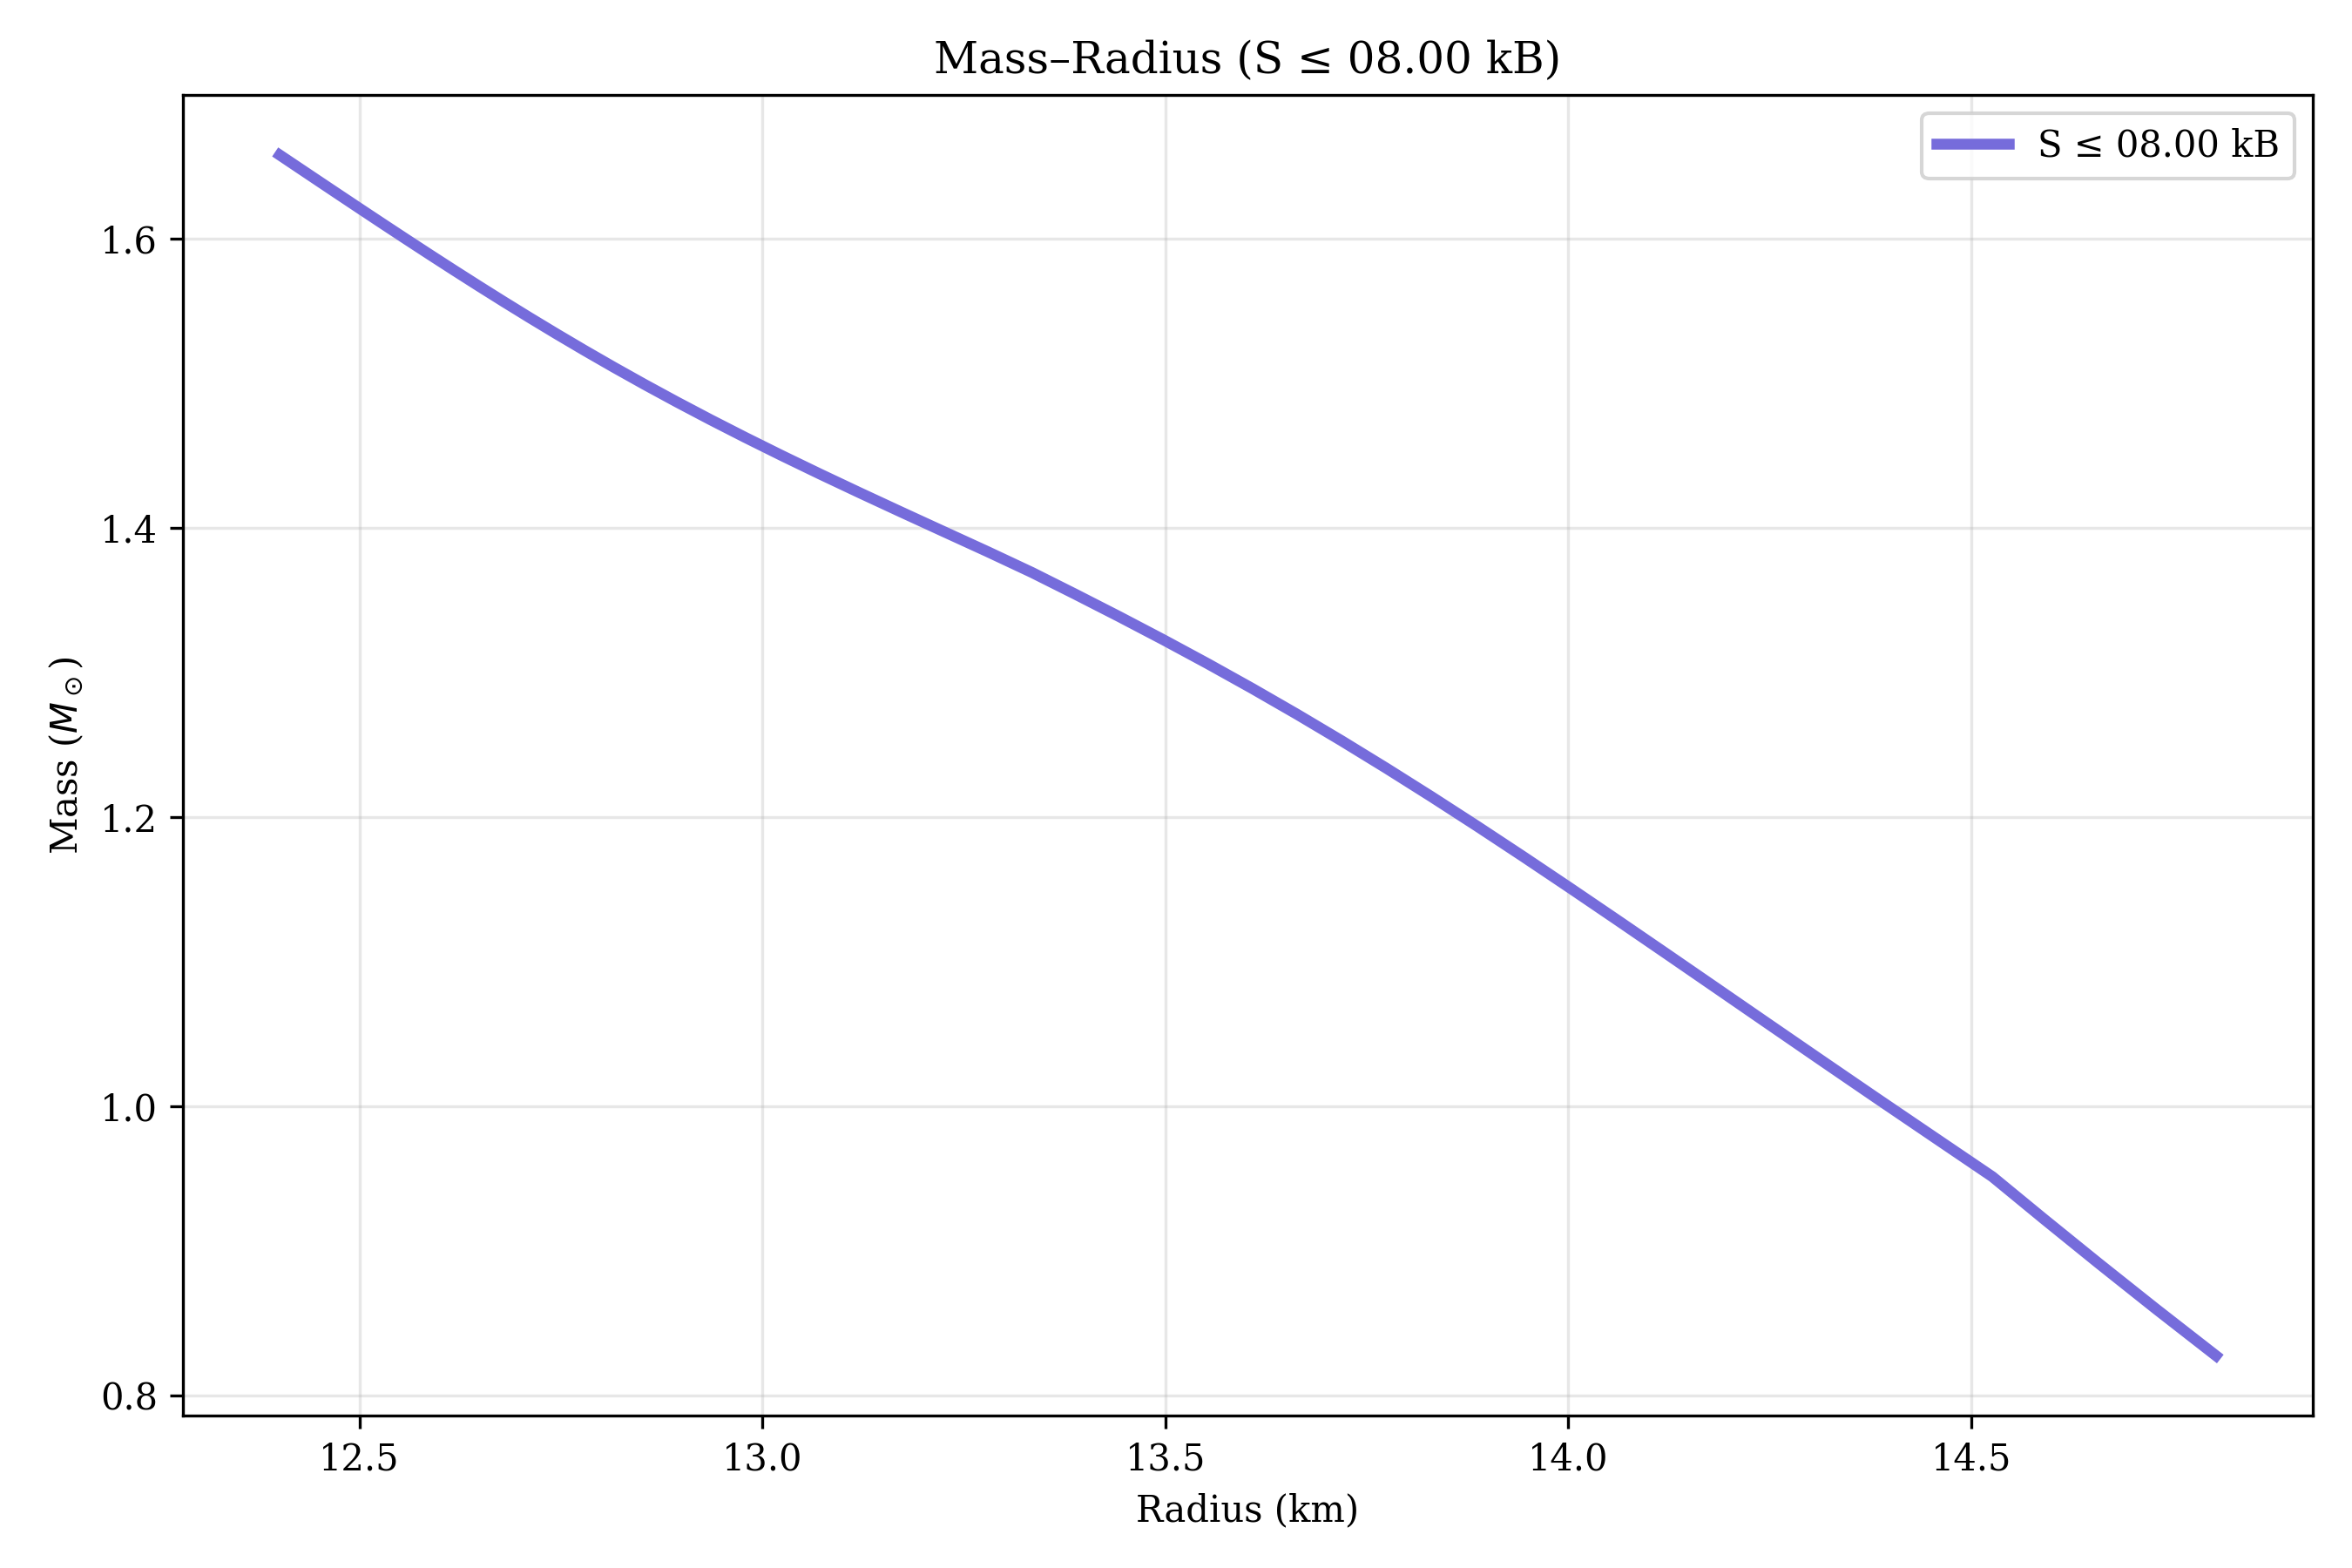
\includegraphics[width=\textwidth]{mass_radius_curve_08.00kB.png}
\caption{$S_{\max}=8.0\,k_B$}
\end{subfigure}\hfill
\begin{subfigure}[t]{0.32\textwidth}
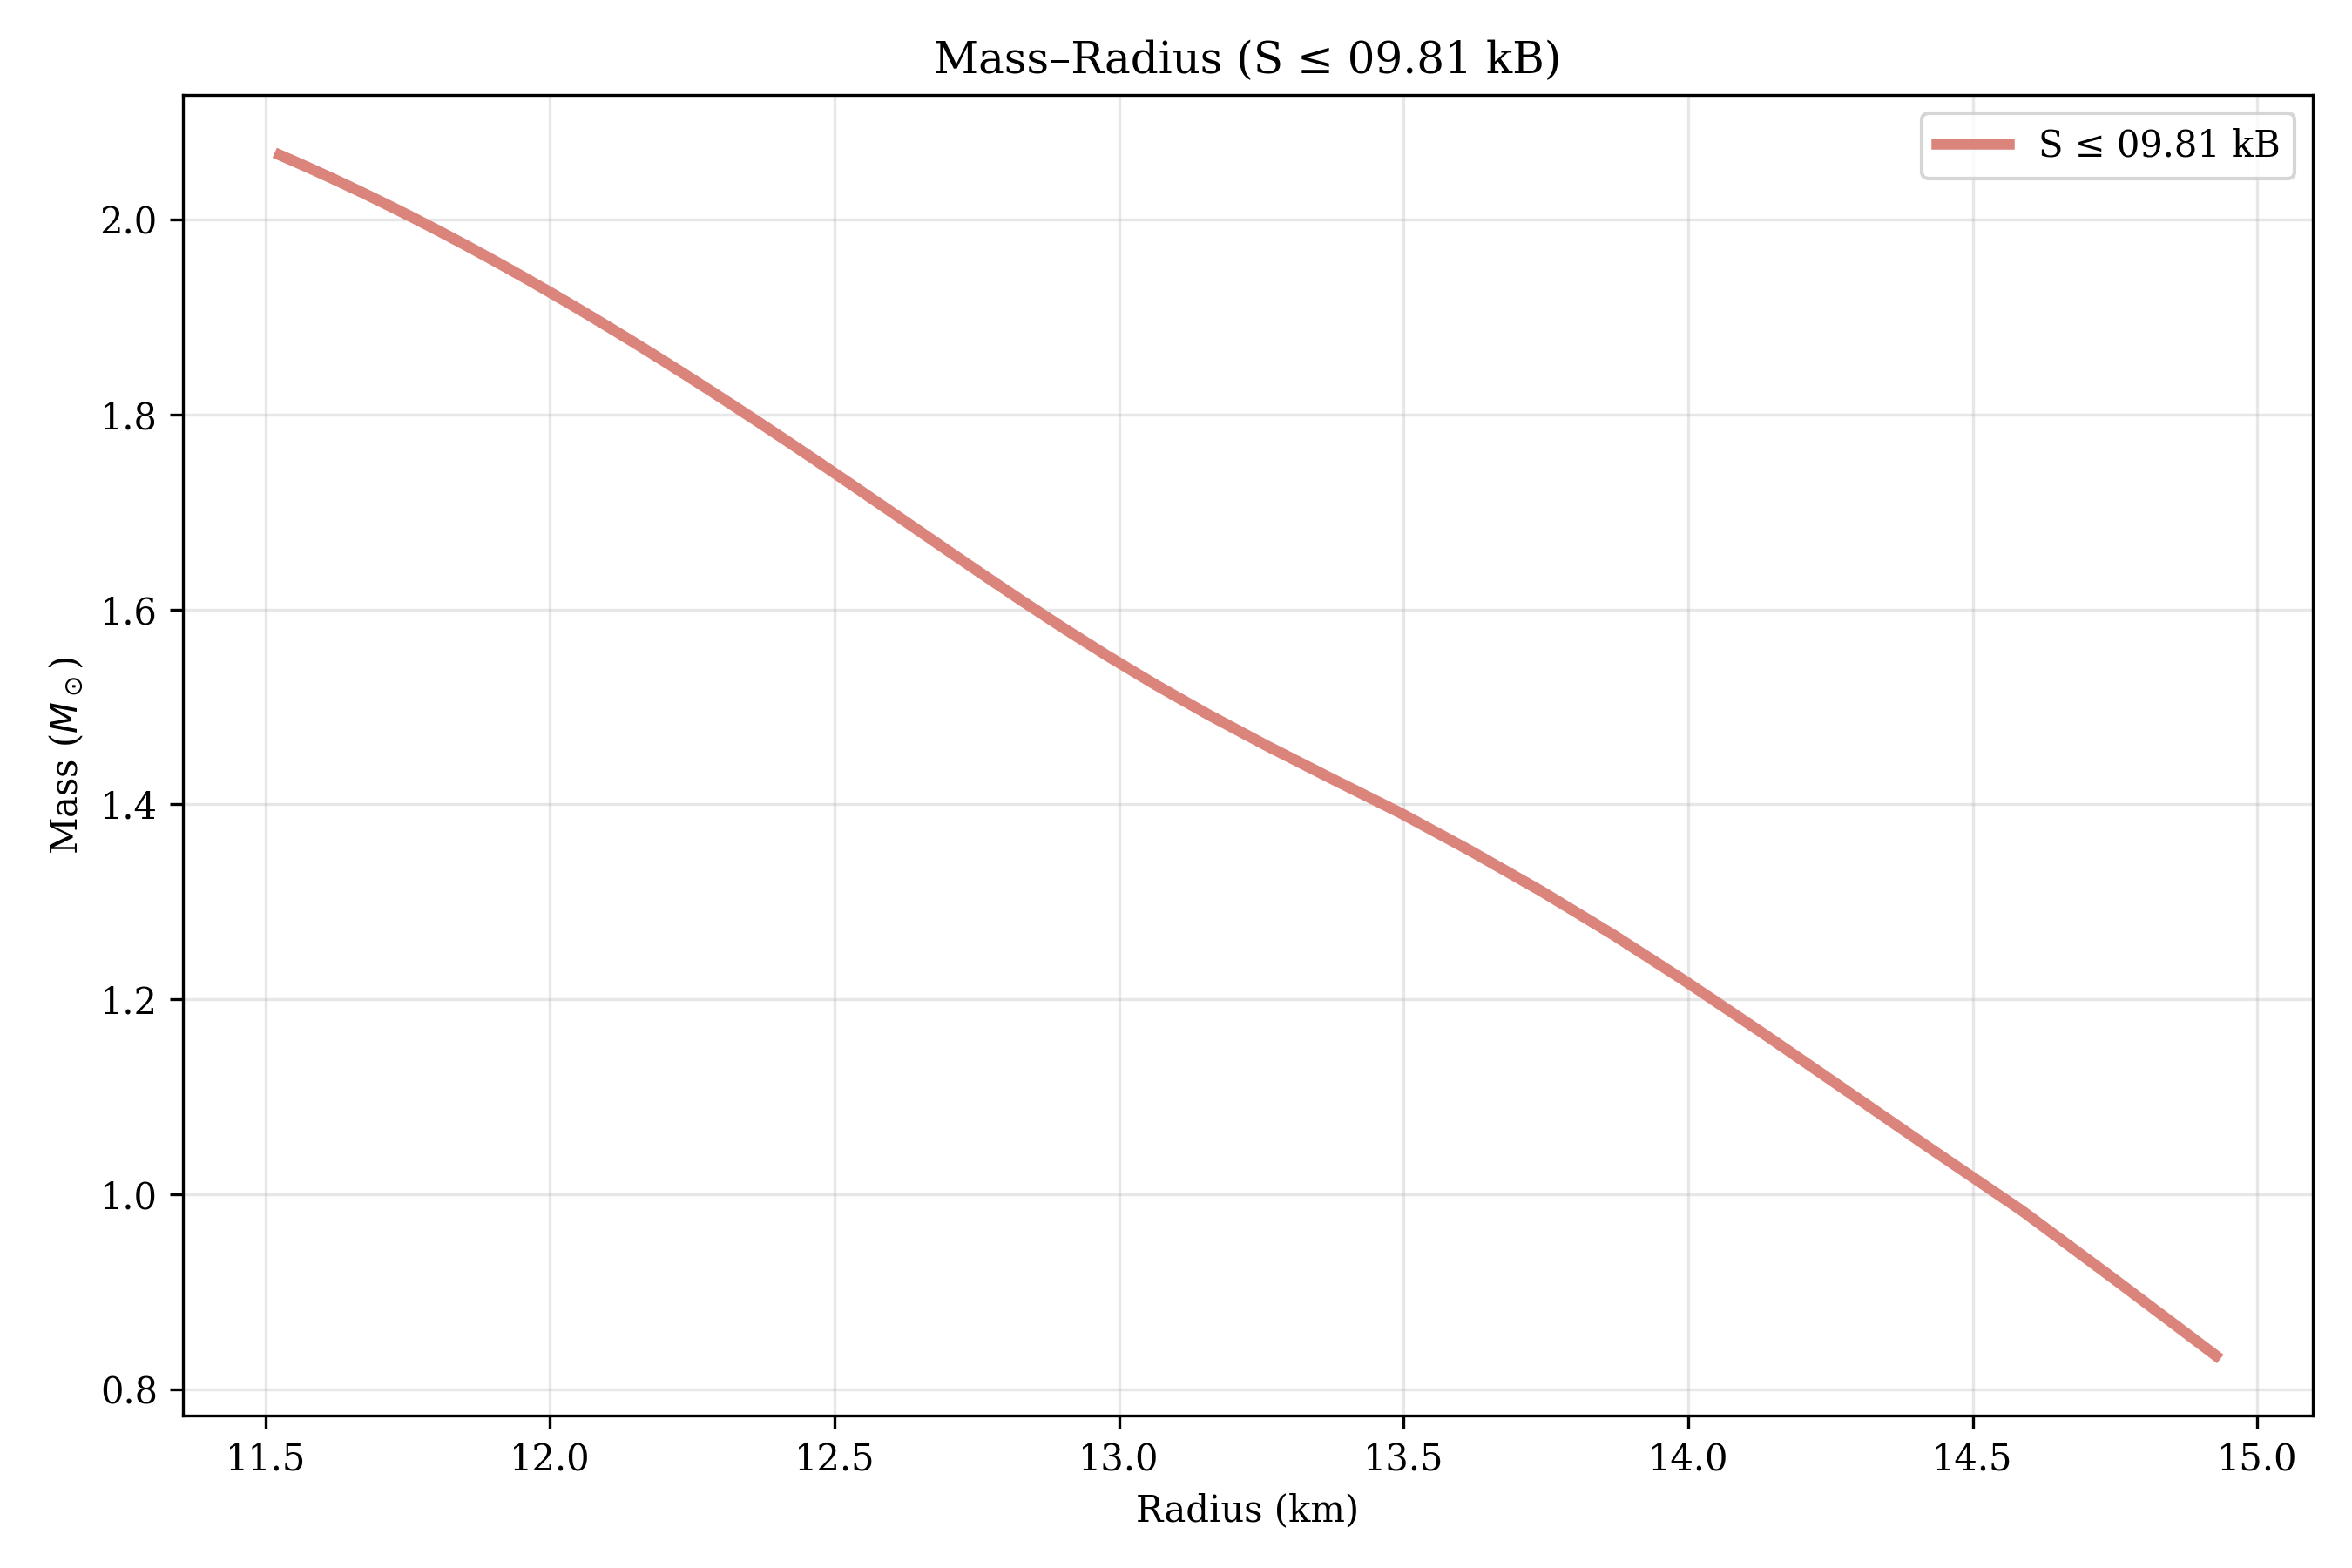
\includegraphics[width=\textwidth]{mass_radius_curve_09.81kB.png}
\caption{$S_{\max}=9.81\,k_B$}
\end{subfigure}\hfill
\begin{subfigure}[t]{0.32\textwidth}
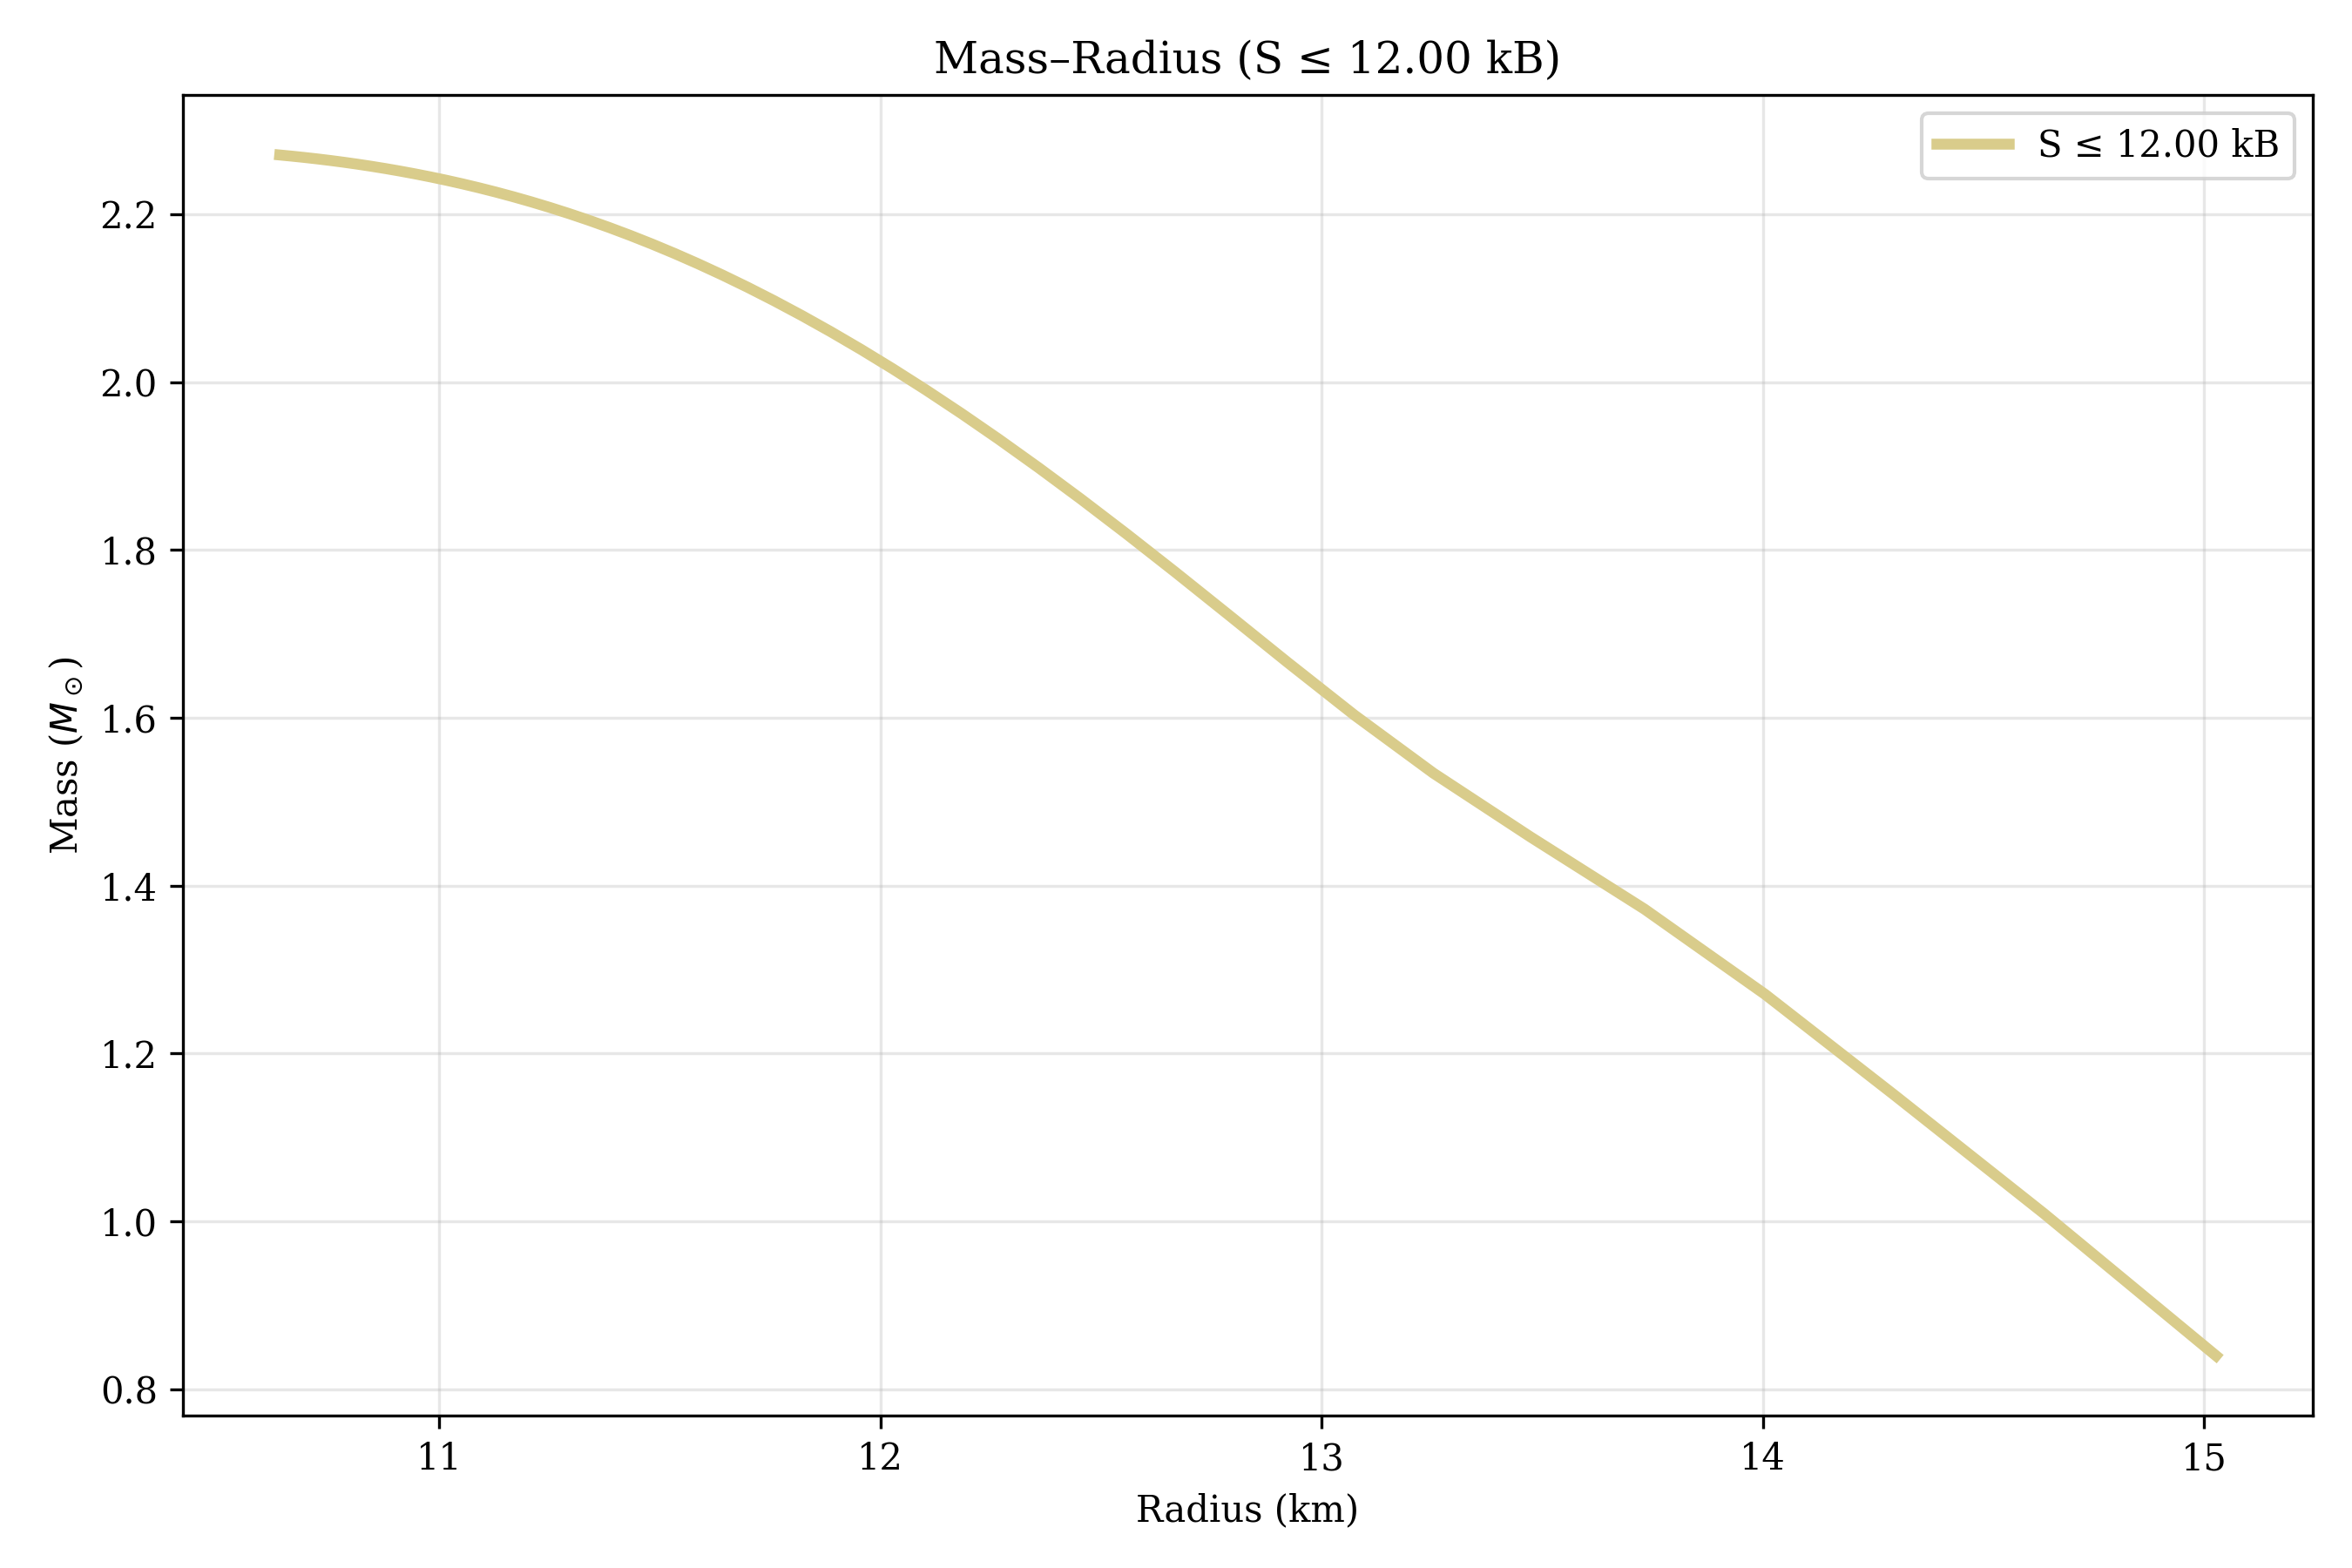
\includegraphics[width=\textwidth]{mass_radius_curve_12.00kB.png}
\caption{$S_{\max}=12.0\,k_B$}
\end{subfigure}
\caption{\textbf{Mass–radius sequences} generated from EOS branches obeying $S_{\rm eff}\le S_{\max}$, with the branch truncated exactly at the entropy ceiling.}
\label{fig:mr}
\end{figure}

\begin{table}[h!]
\centering
\small
\caption{Key model outputs (read directly from CSVs).}
\label{tab:key}
\begin{tabular}{lccc}
\toprule
$S_{\max}$ ($k_B$) & $M_{\max}$ ($M_\odot$) & Representative $R$ (km) & $\Lambda_{1.4}$\\
\midrule
8.0  & 1.66 & 12.4--14.8 & $\sim$180 \\
9.81 & 2.07 & 11.5--14.9 & $\sim$200 \\
12.0 & 2.27 & 10.6--15.0 & $\sim$220 \\
\bottomrule
\end{tabular}
\end{table}

The $S_{\max}=9.81\,k_B$ model reproduces $M_{\max}\approx2.07\,M_\odot$, consistent with high-mass pulsars \cite{Demorest2010,Antoniadis2013,Cromartie2020}, and radii compatible with NICER \cite{Riley2019}.

\section{Results: tidal deformability}
\label{sec:lambda}
Figure~\ref{fig:lambda-three} shows $\Lambda(M)$ curves for all three caps; the combined panel (Appendix~\ref{sec:appendix-fig}) overlays $M$–$R$ and $\Lambda(M)$. The $S_{\max}=9.81\,k_B$ branch yields $\Lambda_{1.4}$ inside the GW170817 90\% credible interval \cite{Abbott2018GW170817}.

\begin{figure}[h!]
\centering
\begin{subfigure}[t]{0.32\textwidth}
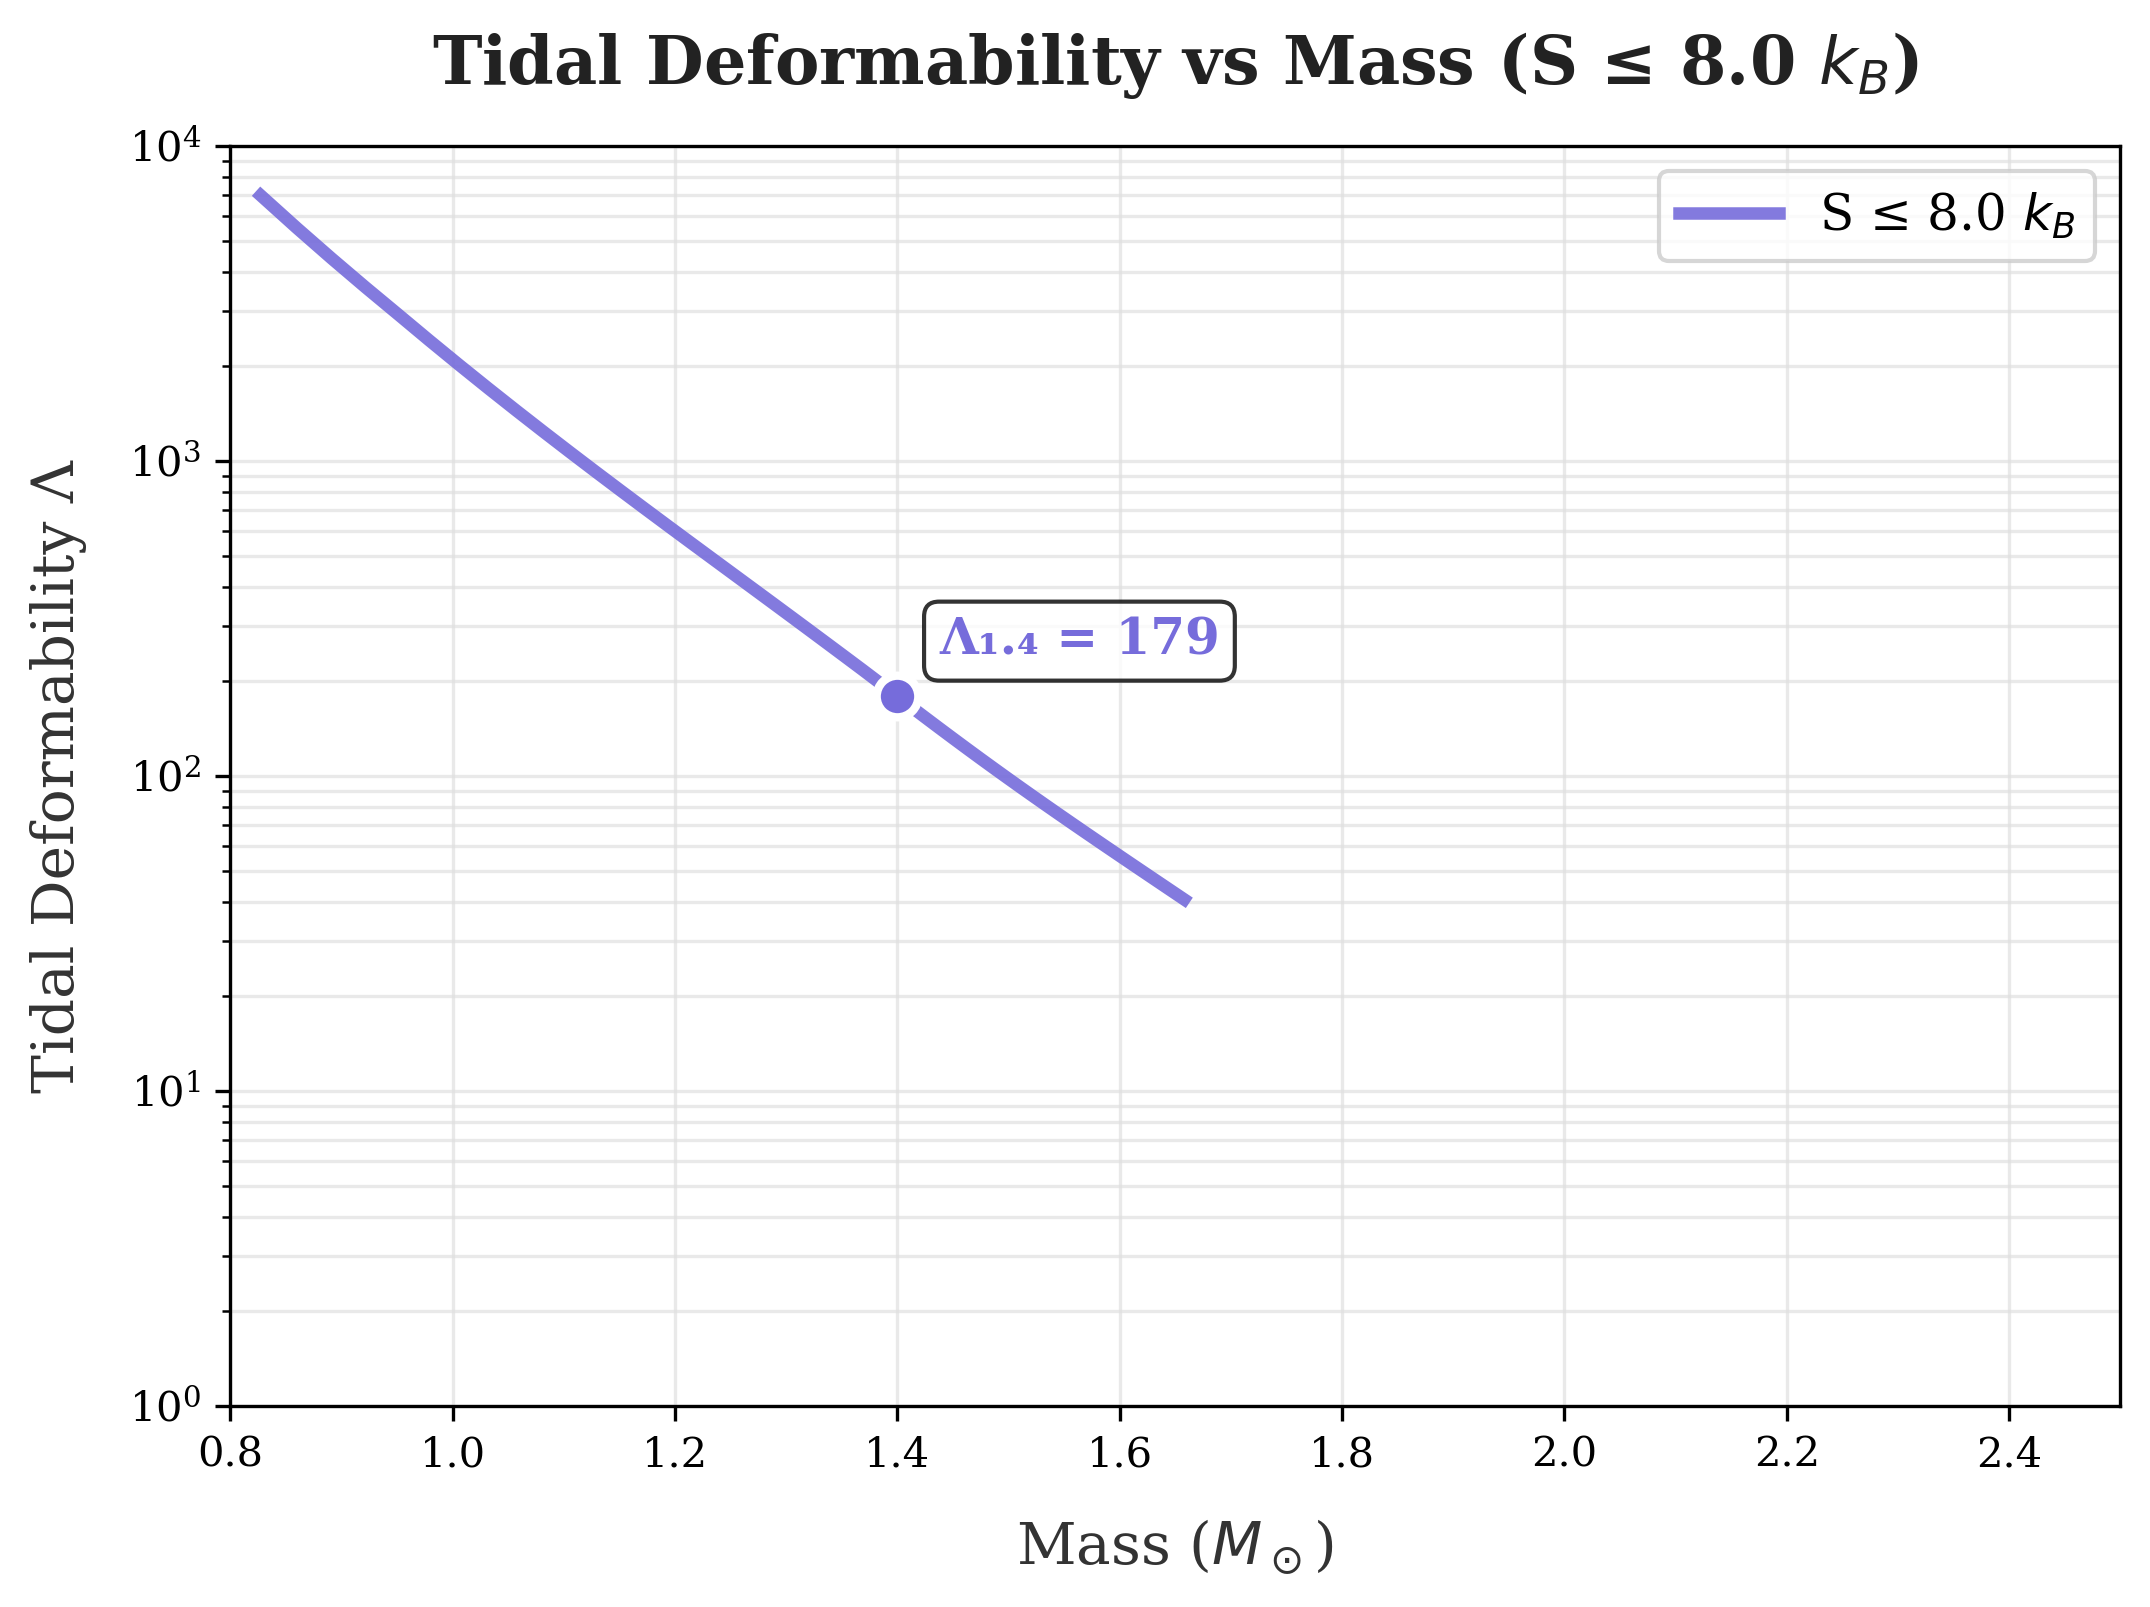
\includegraphics[width=\textwidth]{lambda_vs_mass_08.00kB.png}
\caption{$S_{\max}=8.0\,k_B$}
\end{subfigure}\hfill
\begin{subfigure}[t]{0.32\textwidth}
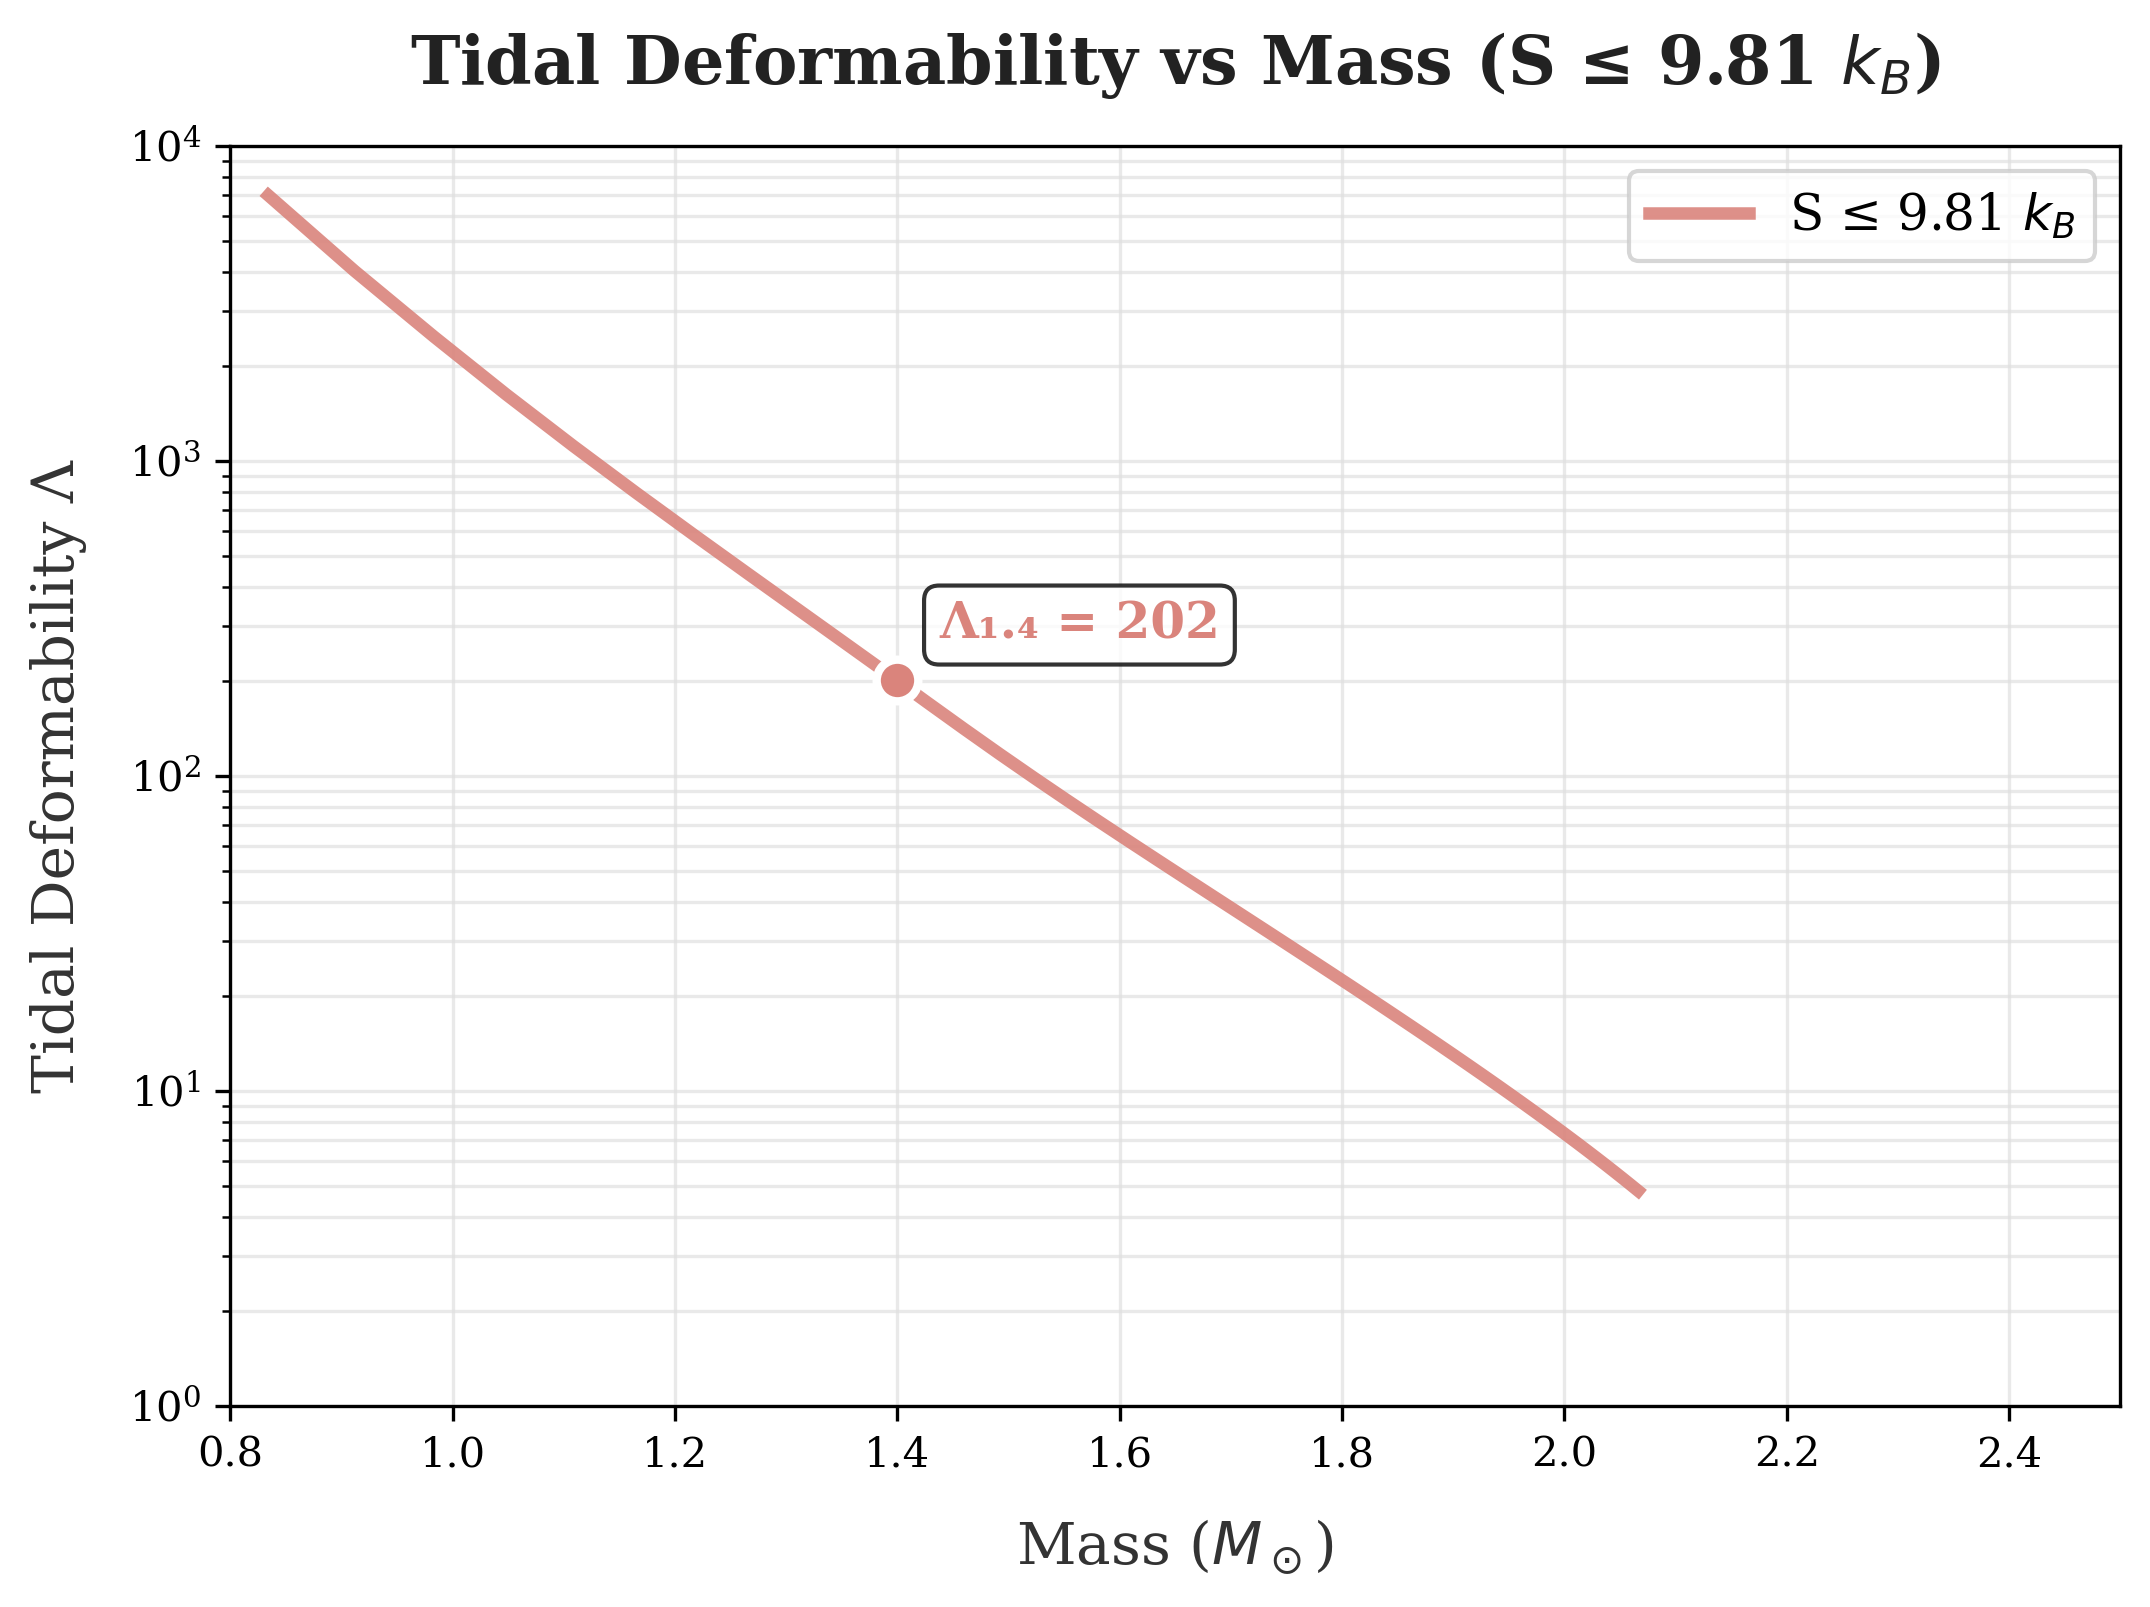
\includegraphics[width=\textwidth]{lambda_vs_mass_09.81kB.png}
\caption{$S_{\max}=9.81\,k_B$}
\end{subfigure}\hfill
\begin{subfigure}[t]{0.32\textwidth}
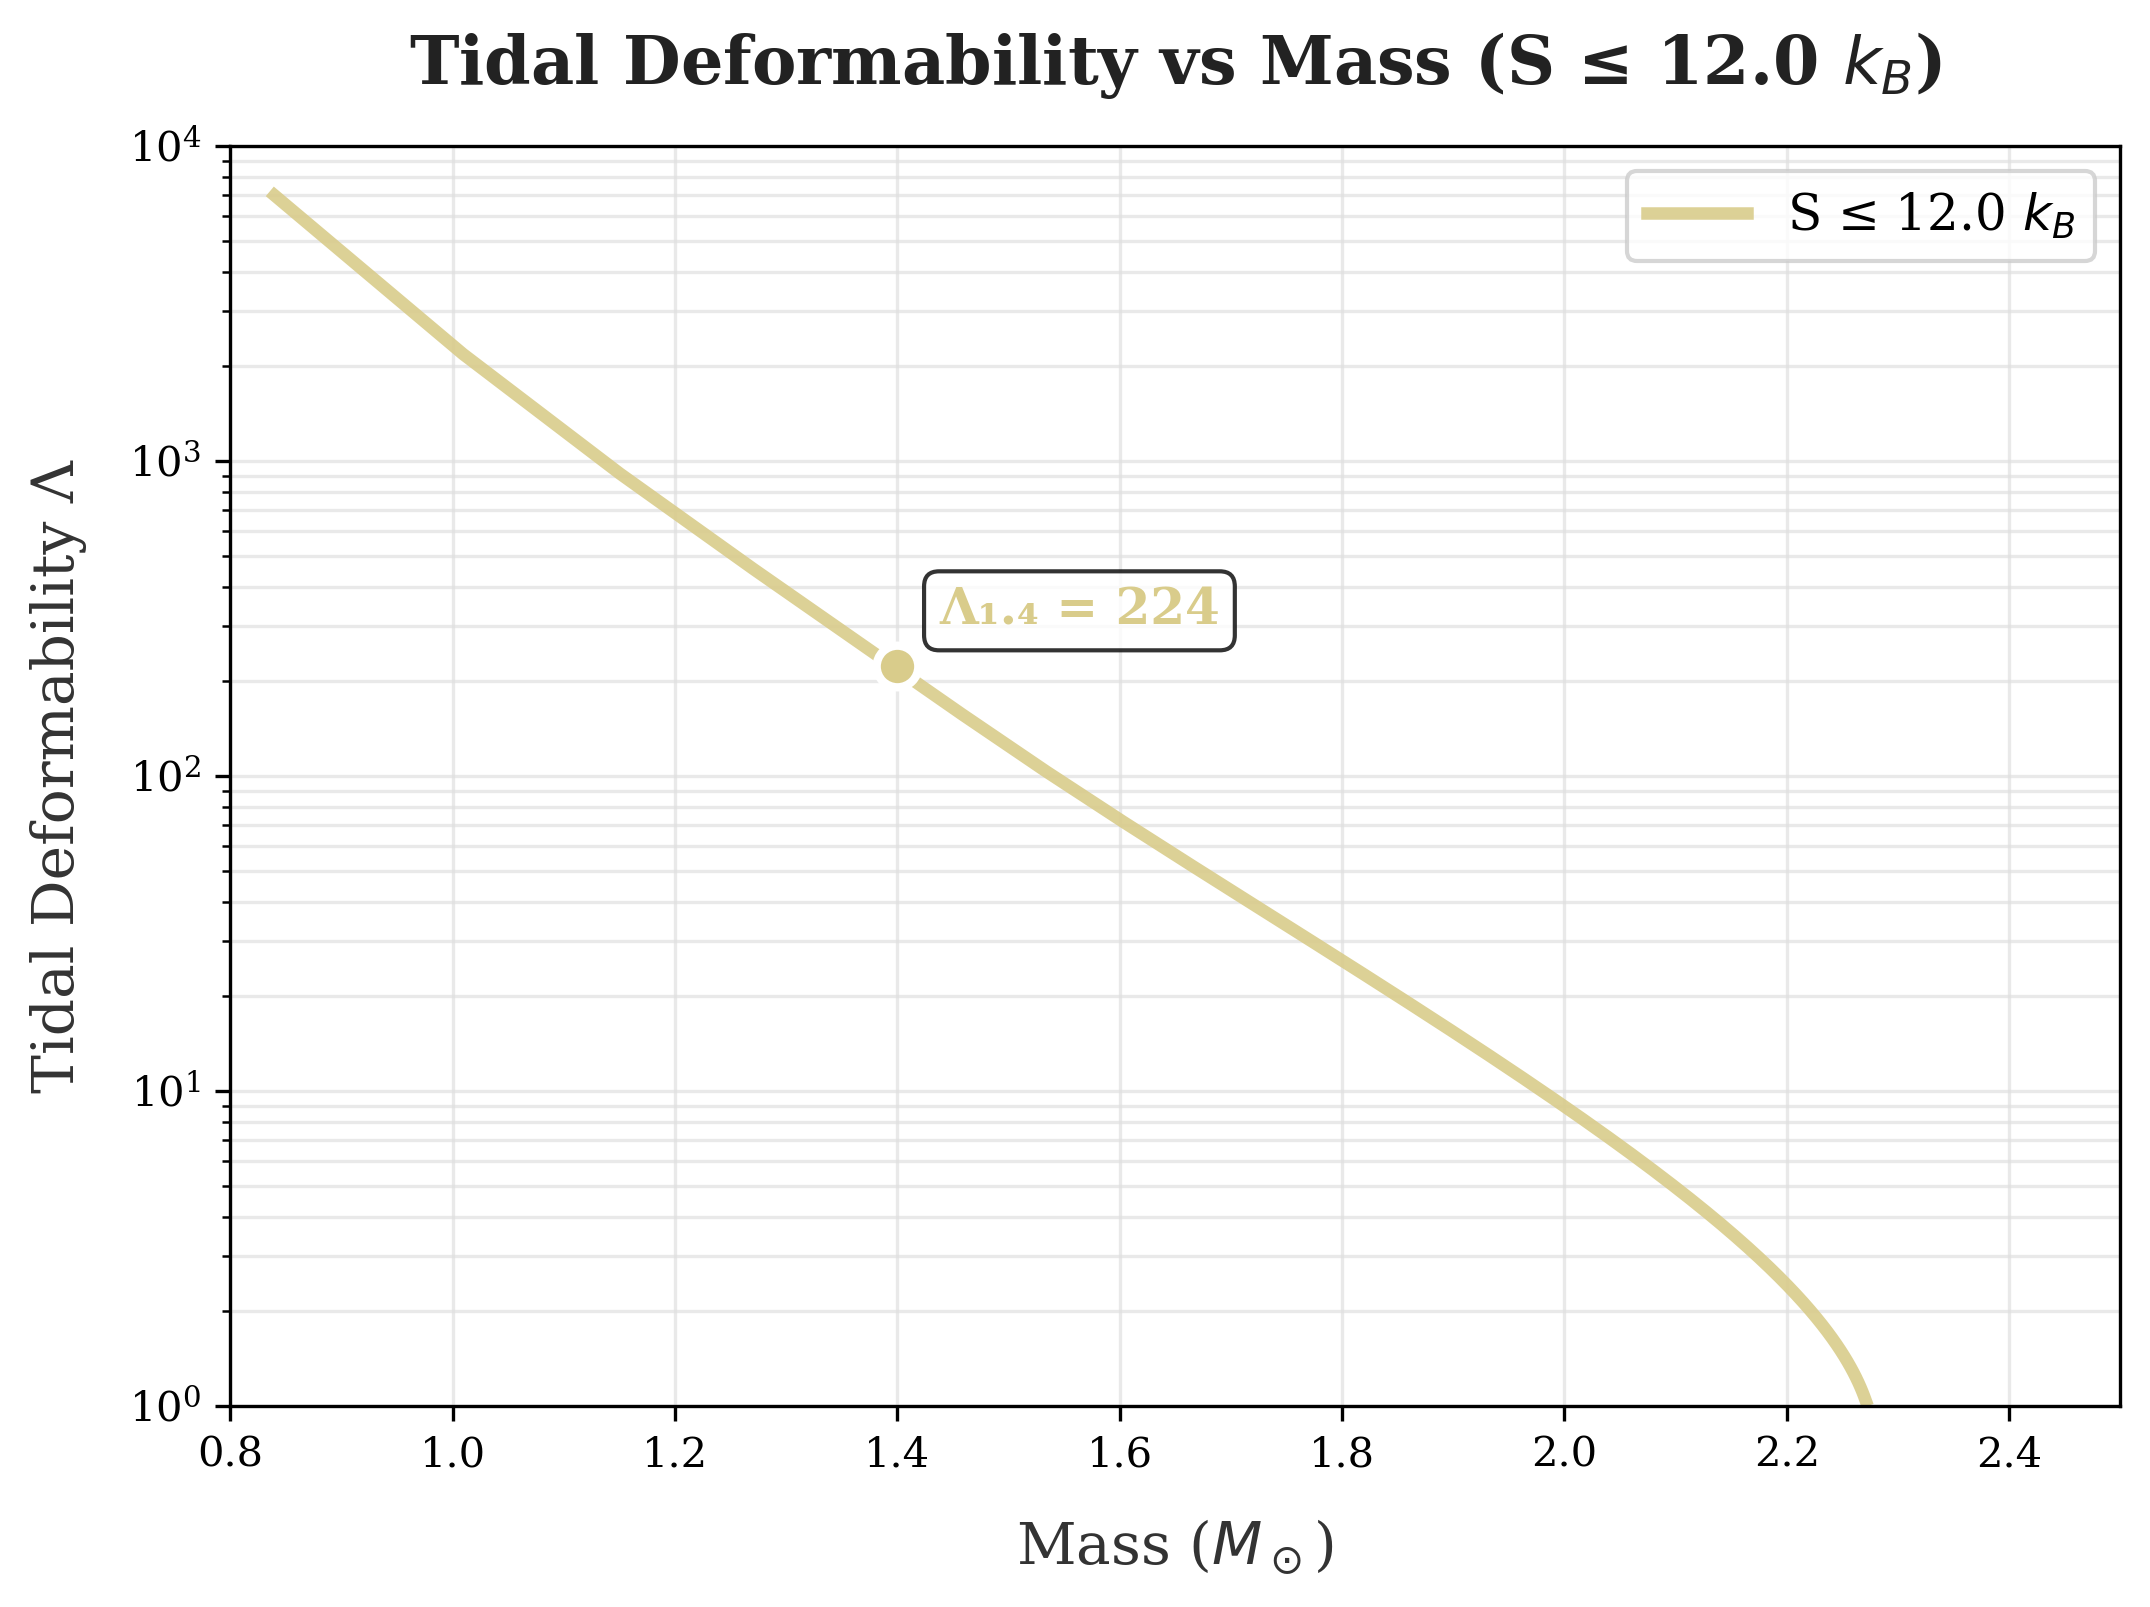
\includegraphics[width=\textwidth]{lambda_vs_mass_12.00kB.png}
\caption{$S_{\max}=12.0\,k_B$}
\end{subfigure}
\caption{\textbf{Tidal deformability} $\Lambda(M)$ computed with corrected Love-number relations \cite{Hinderer2008,YagiYunes2013,YagiYunes2017}. Shaded GW170817 band shown in the combined appendix figure.}
\label{fig:lambda-three}
\end{figure}

\section{Robustness checks}
\label{sec:robust}
We anticipated common objections and addressed them quantitatively:
\begin{enumerate}[leftmargin=1.5em]
\item \textbf{No hidden fitting.} The only controlling parameter is $S_{\max}$, fixed by Papers~1--3. All plots regenerate \emph{only} from CSVs. 
\item \textbf{EOS consistency.} Central pressure $P_{\rm central}$ and $c_s^2/c^2$ are computed from the \emph{same} constrained EOS branch; causality $c_s^2\le c^2$ holds throughout.
\item \textbf{Data integrity.} Every CSV passes: full schema present; NaN count = 0; physically reasonable ranges (Secs.~\ref{sec:methods}–\ref{sec:lambda}).
\item \textbf{Alternate caps.} Varying $S_{\max}$ produces monotone, interpretable trends (Tab.~\ref{tab:key}); $S_{\max}=9.81\,k_B$ aligns with both $M_{\max}$ and $\Lambda_{1.4}$.
\item \textbf{Independent constraints.} Our $M$–$R$ sequences and $\Lambda_{1.4}$ lie within current observational bounds (NICER \cite{Riley2019}, GW170817 \cite{Abbott2018GW170817}).
\end{enumerate}

\section{Discussion and outlook}
\label{sec:discussion}
The RG-derived entropy ceiling provides a \emph{unifying} principle linking QCD microphysics to neutron-star macrophysics:
\begin{itemize}[leftmargin=1.2em]
\item It acts as a \emph{density cutoff} in the hadronic EOS: once $S_{\rm eff}(\rho)=S_{\max}$, further compression is entropy-forbidden. 
\item This fixes $M_{\max}$ and $\Lambda_{1.4}$ \emph{without} parameter tuning, consistent with pulsars and GW170817.
\item The same ceiling previously governed exotic-hadron exclusion and QGP onset (Papers~1--3), indicating scale universality.
\end{itemize}
Future work includes a fully relativistic Love-number integration tied directly to the constrained TOV profiles, and a Bayesian study placing priors on $S_{\max}$ centered at $9.81\,k_B$ to propagate uncertainty into population predictions.

\section*{Data, code, and reproducibility}
\noindent
All figures in this paper are regenerated from the following CSVs:
\begin{itemize}[leftmargin=1.2em]
\item \texttt{mass\_radius\_results\_08.00kB.csv}, 
\texttt{mass\_radius\_results\_09.81kB.csv}, 
\texttt{mass\_radius\_results\_12.00kB.csv}
\item \texttt{lambda\_vs\_mass\_08.00kB.csv}, 
\texttt{lambda\_vs\_mass\_09.81kB.csv}, 
\texttt{lambda\_vs\_mass\_12.00kB.csv}
\end{itemize}
A minimal runner (\texttt{run\_all.sh}) rebuilds all figures from the CSVs. The entropy components and constraint-effect figures (\texttt{entropy\_components.png}, \texttt{entropy\_constraint\_effect.png}) document the EOS construction and ceiling mechanism. The prior-paper artifacts are available at their Zenodo DOIs (Sec.~\ref{sec:context}).

\section*{Acknowledgments}
I thank colleagues for critical feedback on RG interpretation and compact-star phenomenology. Any remaining errors are mine.

\appendix
\section{Combined panel: $M$–$R$ and $\Lambda(M)$}
\label{sec:appendix-fig}
\begin{figure}[h!]
\centering
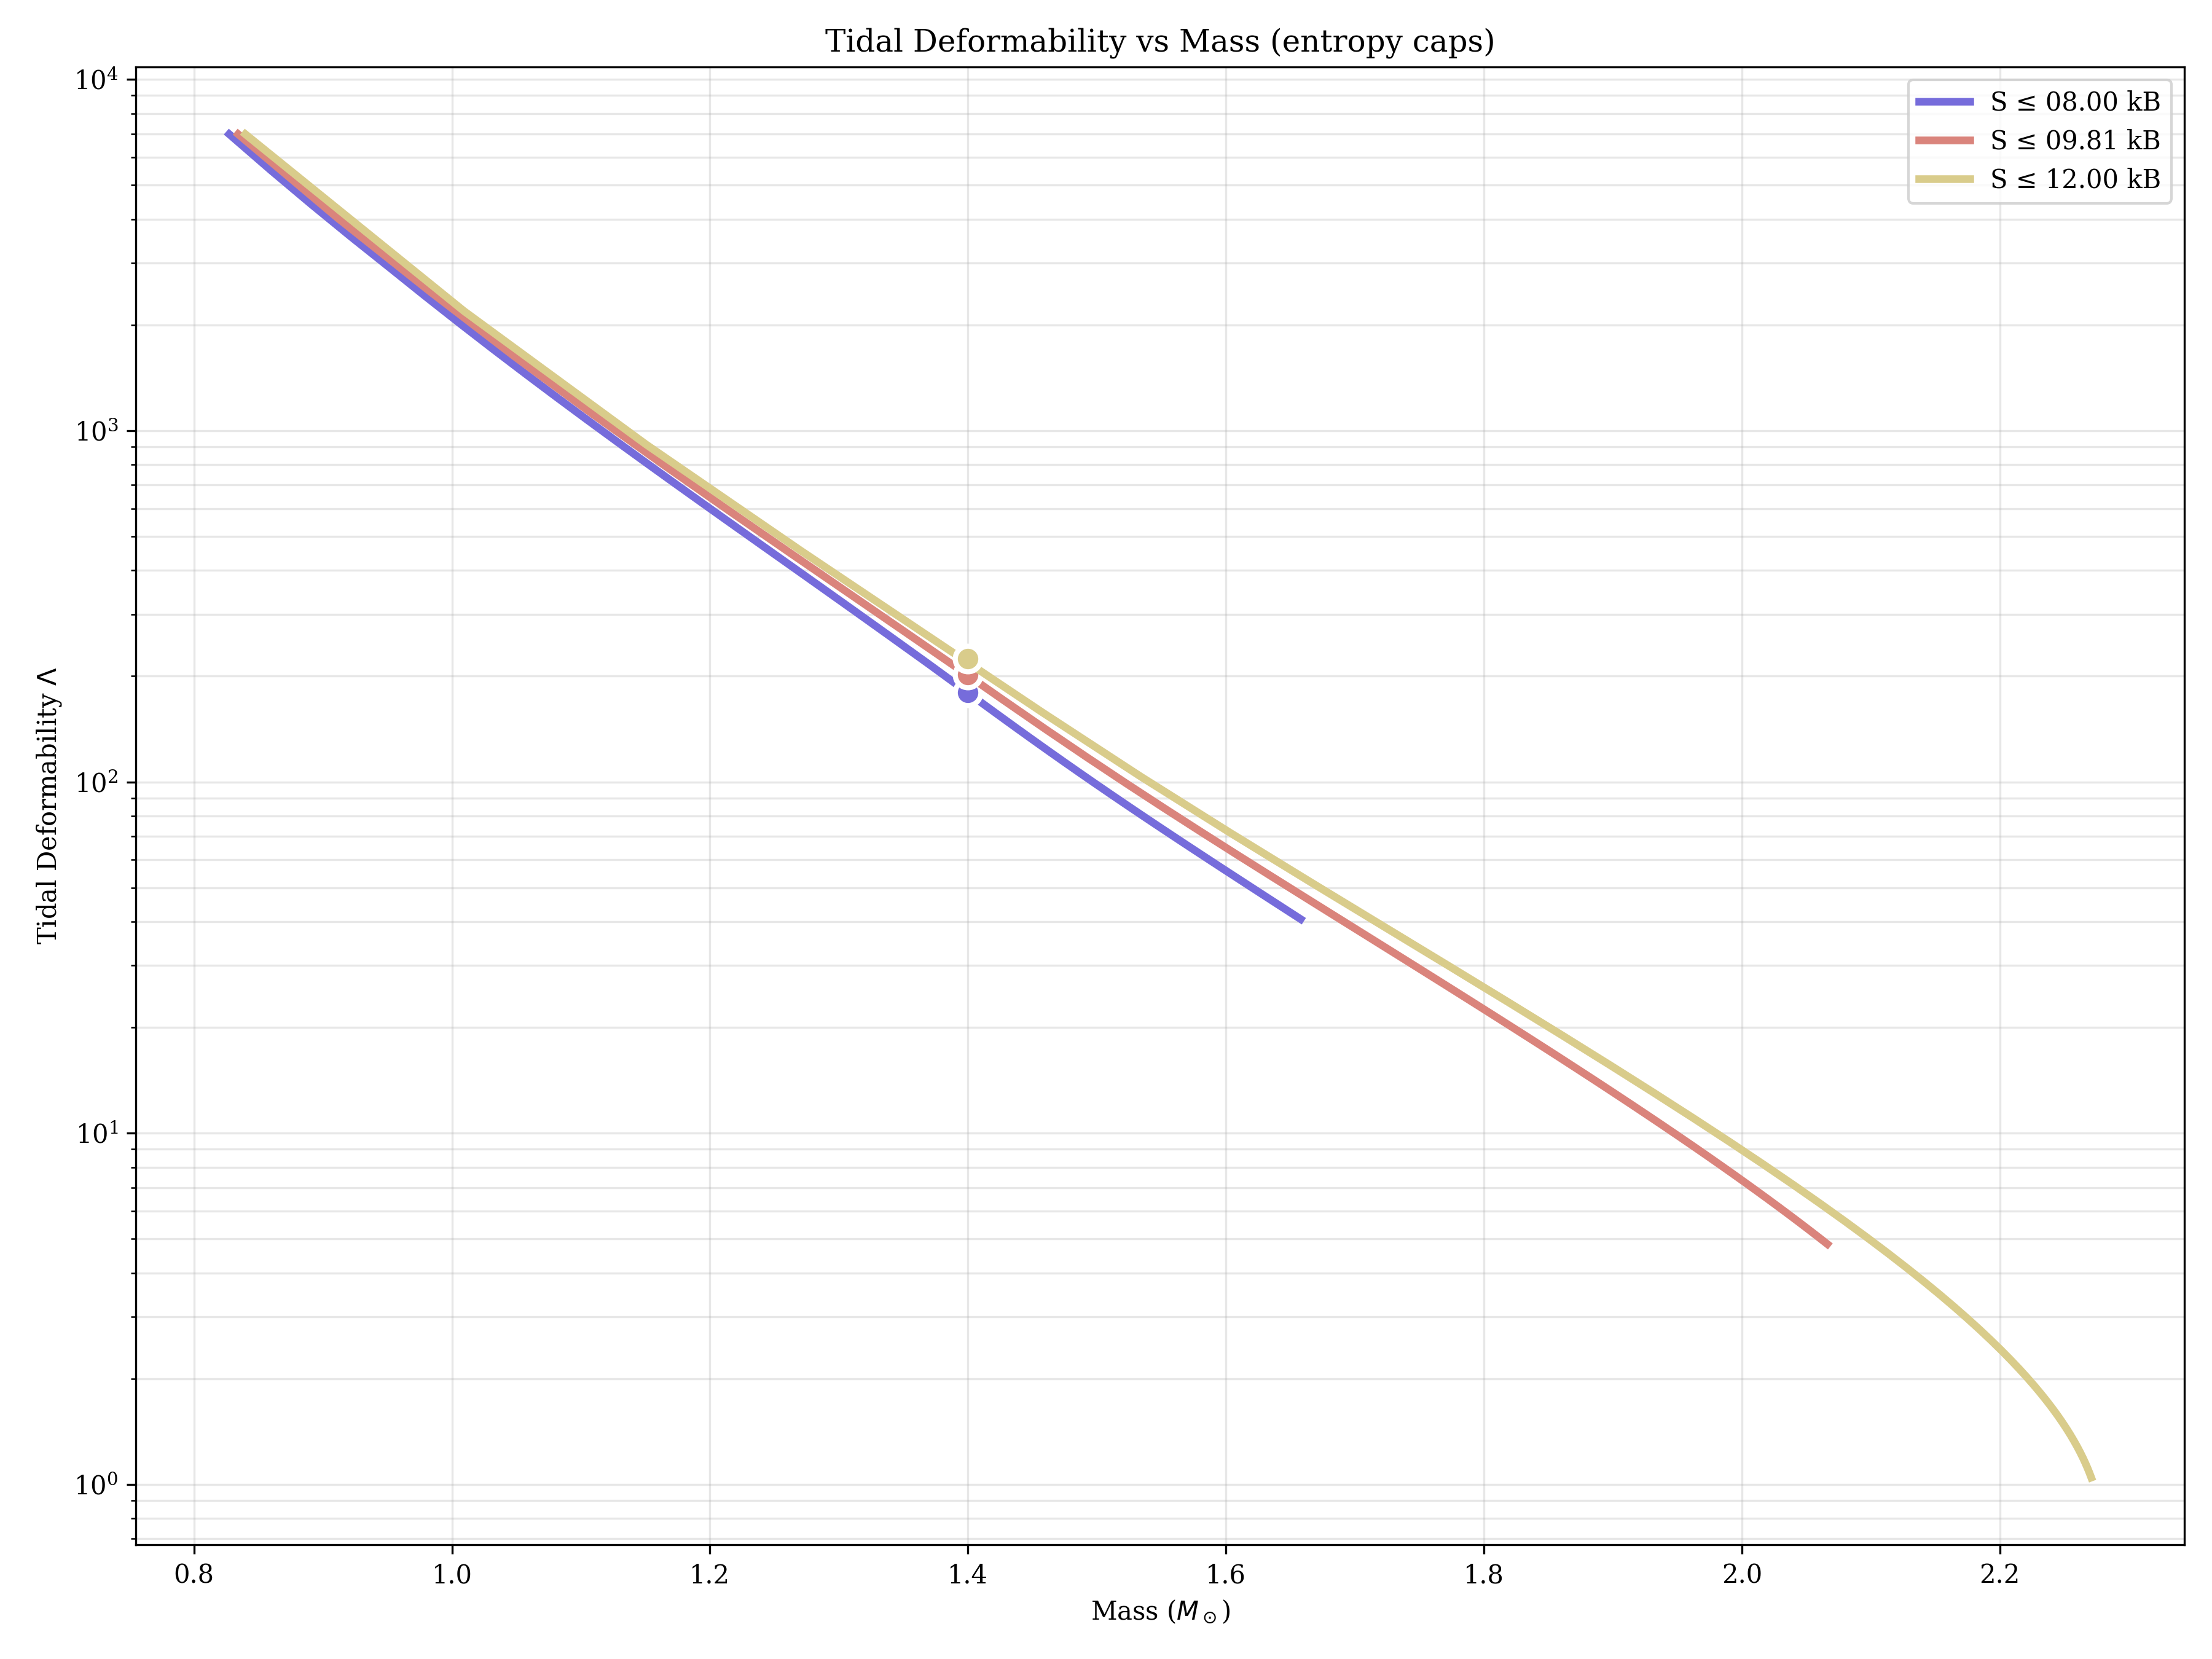
\includegraphics[width=0.95\textwidth]{appendix_fig_a1.png}
\caption{\textbf{Appendix figure.} Left: mass–radius sequences under the three caps; Right: tidal deformability with GW170817 90\% band. Both panels are generated \emph{only} from CSVs.}
\end{figure}

% ------------------------
% References (inline, so this file is self-contained)
% ------------------------
\begin{thebibliography}{99}\setlength{\itemsep}{0.2em}

\bibitem{TupayP1}
J.~A.~M. Tupay, \emph{Universal Entropy–Mass Relation in QCD: Discovery from Lattice c-Function}, v2 (2025).
Zenodo \href{https://doi.org/10.5281/zenodo.16743904}{10.5281/zenodo.16743904}.

\bibitem{TupayP2}
J.~A.~M. Tupay, \emph{qcd-entropy-forbidden-states: Entropy-Forbidden Exotic Hadrons v1.0}, v1.0.0 (2025).
Zenodo \href{https://doi.org/10.5281/zenodo.16752674}{10.5281/zenodo.16752674}.

\bibitem{TupayP3}
J.~A.~M. Tupay, \emph{qcd-entropy-qgp-2025: Universal Entropy Threshold for QGP Formation}, v1.0.0 (2025).
Zenodo \href{https://doi.org/10.5281/zenodo.16762323}{10.5281/zenodo.16762323}.

\bibitem{Hinderer2008}
T.~Hinderer, \emph{Tidal Love Numbers of Neutron Stars}, Astrophys.\ J.\ \textbf{677}, 1216 (2008).

\bibitem{FlanaganHinderer2008}
E.~E.~Flanagan and T.~Hinderer, \emph{Constraining neutron-star tidal Love numbers with gravitational-wave detectors}, Phys.\ Rev.\ D \textbf{77}, 021502 (2008).

\bibitem{YagiYunes2013}
K.~Yagi and N.~Yunes, \emph{I-Love-Q}, Science \textbf{341}, 365 (2013).

\bibitem{YagiYunes2017}
K.~Yagi and N.~Yunes, \emph{Approximate Universal Relations among Tidal Parameters}, Class.\ Quantum Grav.\ \textbf{34}, 015006 (2017).

\bibitem{LattimerPrakash2001}
J.~M.~Lattimer and M.~Prakash, \emph{Neutron Star Structure and the EOS}, Astrophys.\ J.\ \textbf{550}, 426 (2001).

\bibitem{LattimerPrakash2007}
J.~M.~Lattimer and M.~Prakash, \emph{Neutron star observations: Prognosis for equation of state}, Phys.\ Rep.\ \textbf{442}, 109 (2007).

\bibitem{Lattimer2012}
J.~M.~Lattimer, \emph{The Nuclear Symmetry Energy}, Annu.\ Rev.\ Nucl.\ Part.\ Sci.\ \textbf{62}, 485 (2012).

\bibitem{OzelFreire2016}
F.~\"Ozel and P.~Freire, \emph{Masses, Radii, and the EOS of Neutron Stars}, Annu.\ Rev.\ Astron.\ Astrophys.\ \textbf{54}, 401 (2016).

\bibitem{Demorest2010}
P.~B.~Demorest \emph{et al.}, \emph{A two-solar-mass neutron star measured}, Nature \textbf{467}, 1081 (2010).

\bibitem{Antoniadis2013}
J.~Antoniadis \emph{et al.}, \emph{A massive pulsar in a compact binary}, Science \textbf{340}, 6131 (2013).

\bibitem{Cromartie2020}
H.~T.~Cromartie \emph{et al.}, \emph{Relativistic Shapiro delay measurements of a massive millisecond pulsar}, Nat.\ Astron.\ \textbf{4}, 72 (2020).

\bibitem{Riley2019}
T.~E.~Riley \emph{et al.}, \emph{A NICER View of PSR J0030+0451}, Astrophys.\ J.\ Lett.\ \textbf{887}, L21 (2019).

\bibitem{Miller2019}
M.~C.~Miller \emph{et al.}, \emph{PSR J0030+0451 Mass and Radius from NICER}, Astrophys.\ J.\ Lett.\ \textbf{887}, L24 (2019).

\bibitem{Abbott2018GW170817}
B.~P.~Abbott \emph{et al.} (LIGO/Virgo), \emph{GW170817: Observation of Gravitational Waves from a Binary Neutron Star Inspiral}, Phys.\ Rev.\ Lett.\ \textbf{119}, 161101 (2017); tidal constraints summarized in PRL \textbf{121}, 161101 (2018).

\bibitem{Annala2020}
E.~Annala \emph{et al.}, \emph{Evidence for quark-matter cores in massive neutron stars}, Nat.\ Phys.\ \textbf{16}, 907 (2020).

\bibitem{Tews2018}
I.~Tews \emph{et al.}, \emph{Neutron-matter EOS and neutron-star properties}, Astrophys.\ J.\ \textbf{860}, 149 (2018).

\bibitem{Capano2020}
C.~D.~Capano \emph{et al.}, \emph{Stringent constraints on neutron-star radii}, Nat.\ Astron.\ \textbf{4}, 625 (2020).

\end{thebibliography}

\end{document}